\documentclass[11pt]{beamer}
%
% Choose how your presentation looks.
%
% For more themes, color themes and font themes, see:
% http://deic.uab.es/~iblanes/beamer_gallery/index_by_theme.html
%
	\definecolor{bostonuniversityred}{rgb}{0.8, 0.0, 0.0}
\mode<presentation>
{
  \usetheme{Madrid}      % or try Darmstadt, Madrid, Warsaw, ...
  \usecolortheme{beaver} % or try albatross, beaver, crane, ...
  \usefonttheme{default}  % or try serif, structurebold, ...
  \setbeamertemplate{navigation symbols}{}
  \setbeamertemplate{caption}[numbered]
} 
%\usepackage{pifont}
\documentclass[tikz]{standalone}
\usepackage{neuralnetwork}
\usepackage{qrcode}
\usepackage{listings}
\usepackage{euler}
\usepackage{bbm}
\usetheme[secheader]{Boadilla}
\usecolortheme[named=bostonuniversityred]{structure}
\usepackage[bookmarks]{hyperref}
\usepackage[backend=bibtex]{biblatex}
\setbeamercolor{title}{parent=author in head/foot}
\usepackage{braket}
\usepackage{amsmath,amsfonts,amsthm,bm}
\addbibresource{bibliography.bib}
\newtheorem*{remark}{Remark}
\usepackage[italian]{babel}
\usepackage[utf8x]{inputenc}
\usebackgroundtemplate{\includegraphics[width=\paperwidth]{Pic/Cover_image.png}}
\title[Human hacking \& deepfake]{Human hacking \& deepfake: manipolazione tramite social network e IA generativa }}
\author{Marzio De Corato}
\date{\today}

\newcommand{\xin}[2]{$x_#2$}
\newcommand{\xout}[2]{$\hat x_#2$}


\begin{document}

\begin{frame}
\vspace{+6.5 cm}  \titlepage
\end{frame}

\usebackgroundtemplate{ } 

% Uncomment these lines for an automatically generated outline.
\begin{frame}{Outline}
\setcounter{tocdepth}{1}
\begin{center}
\Large
  \tableofcontents
\end{center}
\end{frame}

\section{Motivazione}

\begin{frame}
\begin{center}
\Huge
Motivazione
\end{center}
\end{frame}

\begin{frame}{Cambridge Analytica \cite{CA_pic}}

\begin{center}
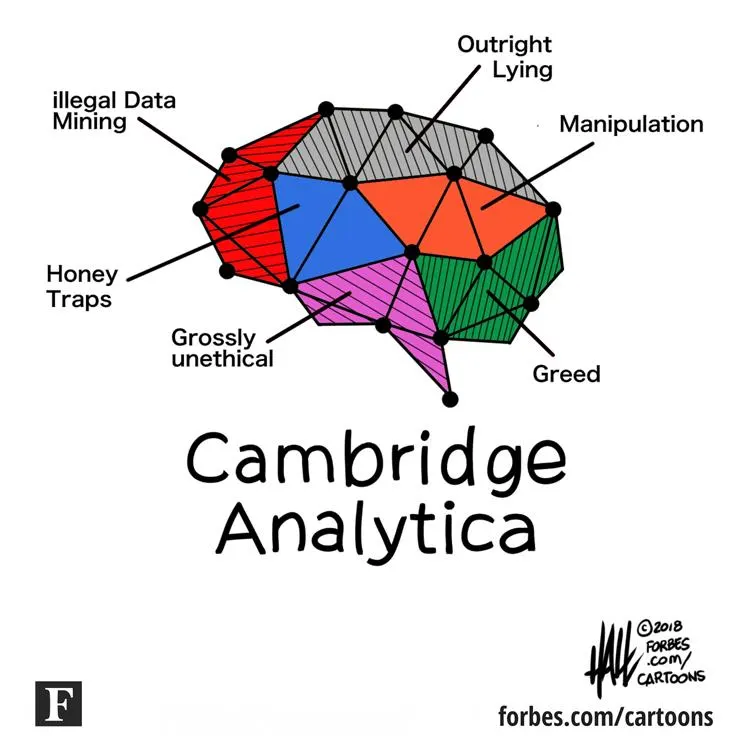
\includegraphics[width=0.8\textwidth]{Pic/CA_pic.png}
\end{center}

\end{frame}

\begin{frame}{Cambridge Analytica \cite{CA_timeline}}

\begin{center}
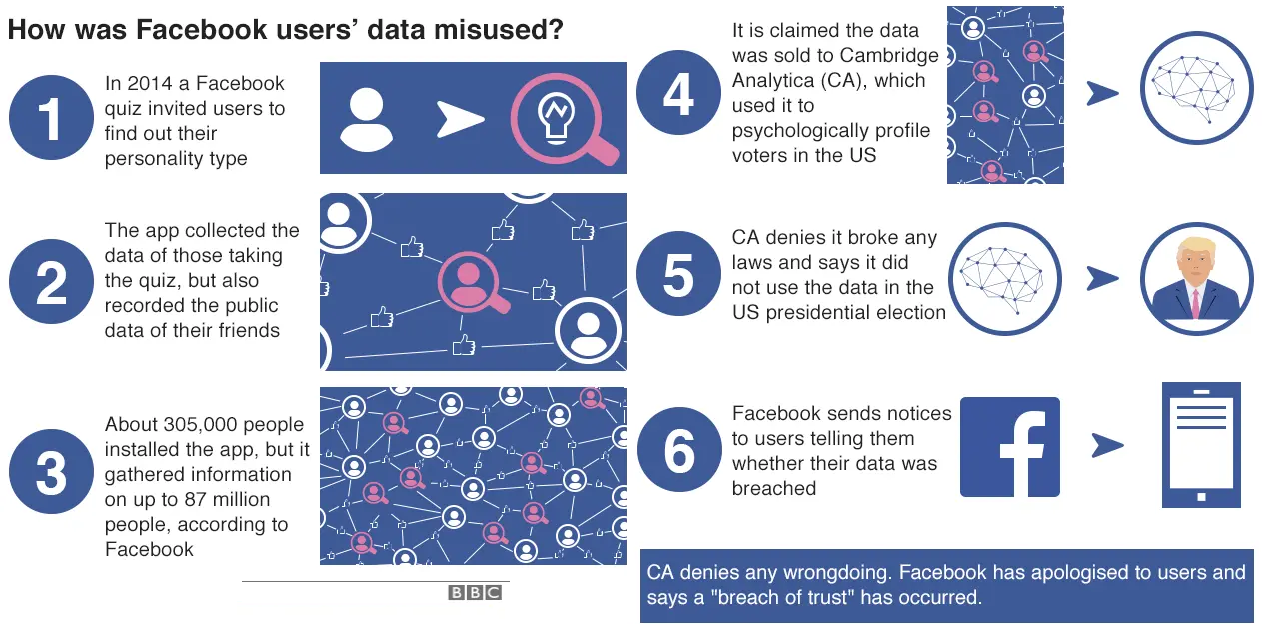
\includegraphics[width=0.8\textwidth]{Pic/cambridge_analitica_timeline.png}
\end{center}

\end{frame}


\begin{frame}{Cambridge Analytica \cite{CA_it2}}

\begin{center}
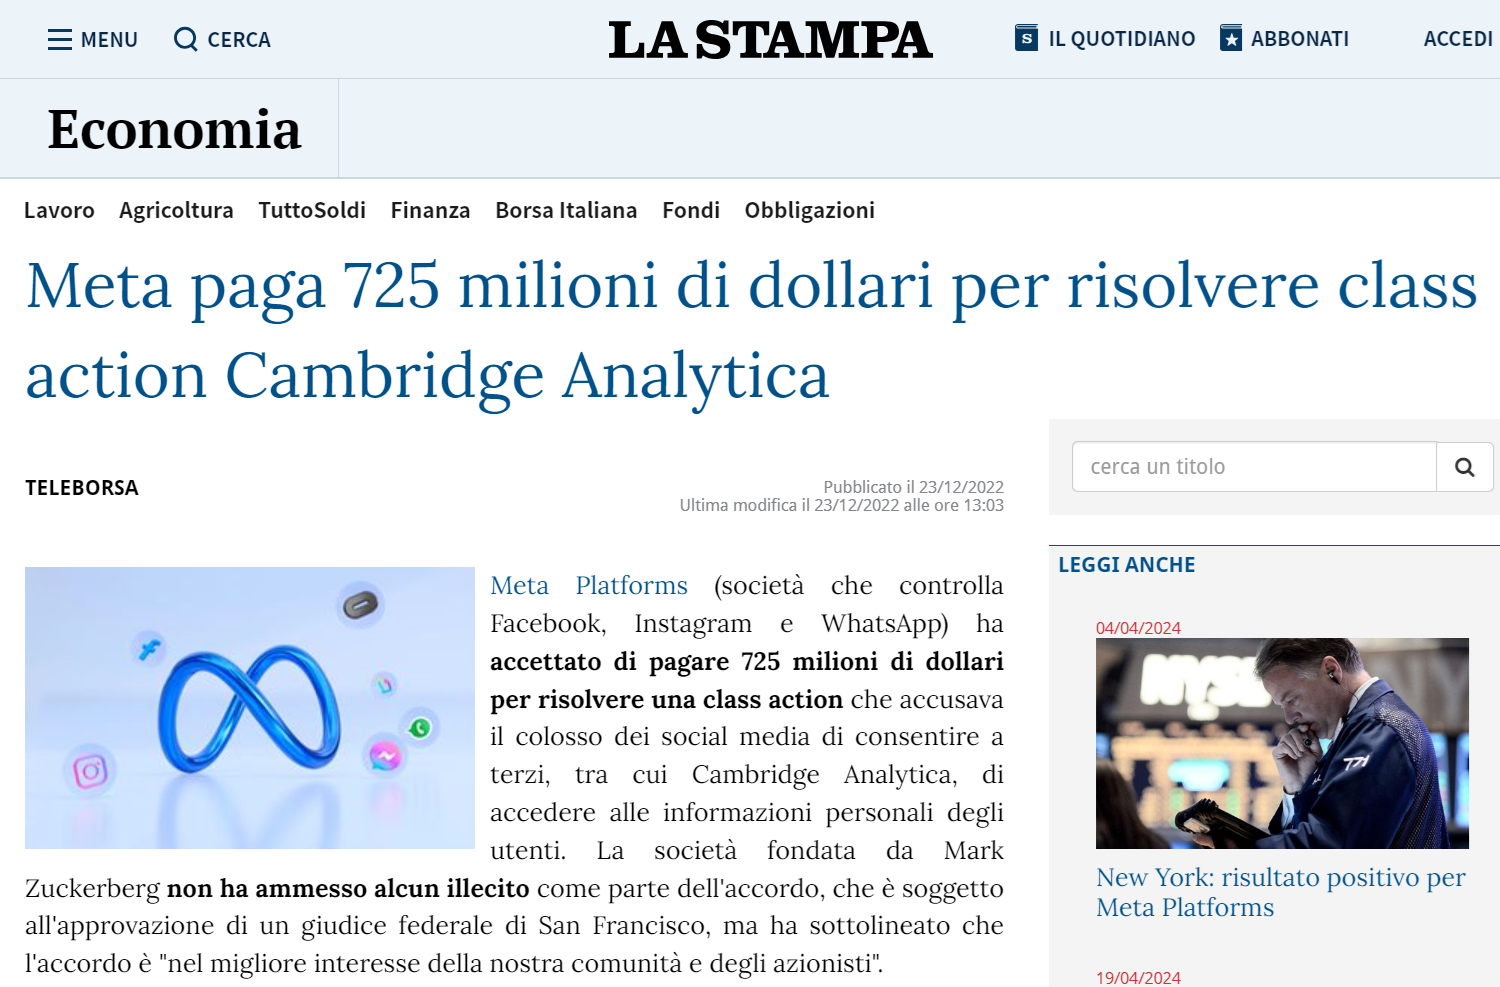
\includegraphics[width=0.8\textwidth]{Pic/FB_CA.png}
\end{center}

\end{frame}

\begin{frame}{Cambridge Analytica \cite{CA_it}}

\begin{center}
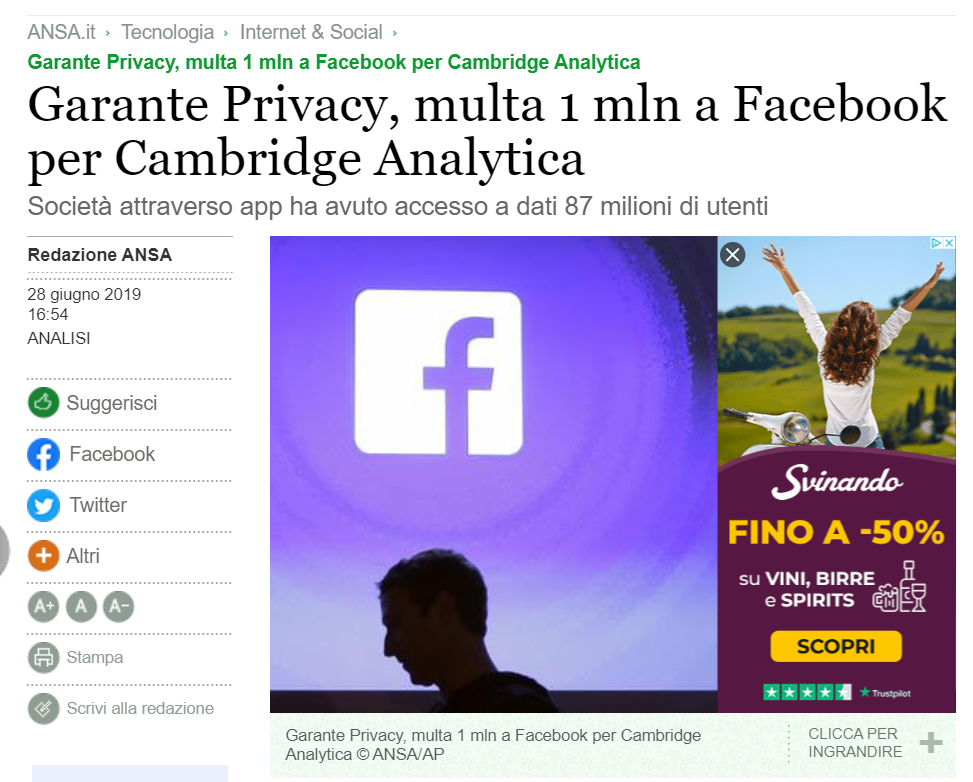
\includegraphics[width=0.8\textwidth]{Pic/FA_CA_ITA.png}
\end{center}

\end{frame}


\begin{frame}{Cambridge Analytica \cite{CA_rev}}

\begin{center}
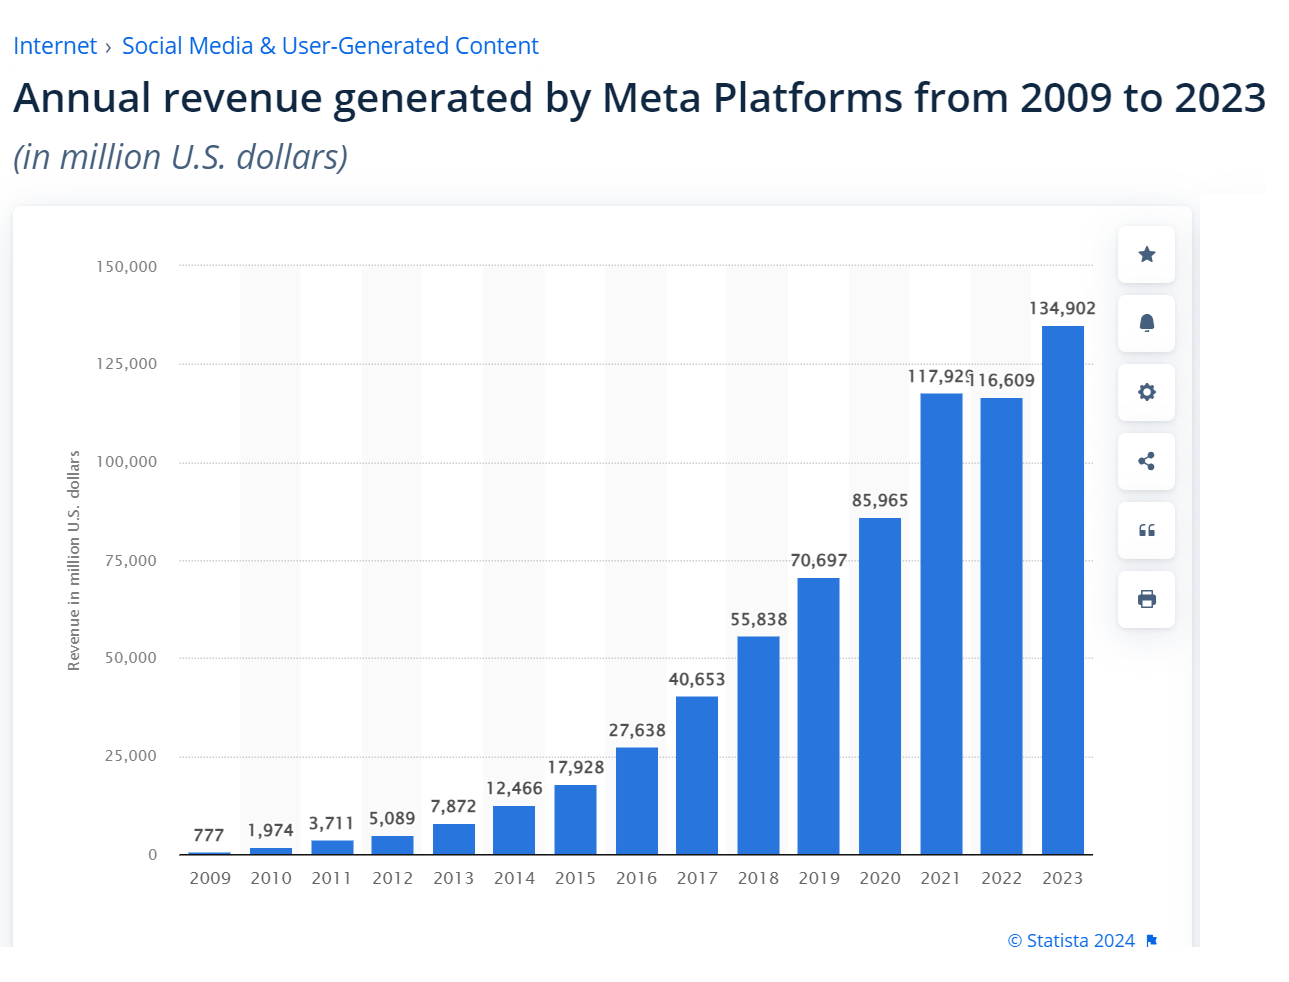
\includegraphics[width=0.8\textwidth]{Pic/FB_REV.png}
\end{center}

\end{frame}

\begin{frame}{Mia Ash}

\begin{center}
\includegraphics[width=0.6\textwidth]{Pic/mia_ASH.png}
\end{center}

\end{frame}


\begin{frame}{Mia Ash \cite{mia_ash_lin}}

\begin{center}
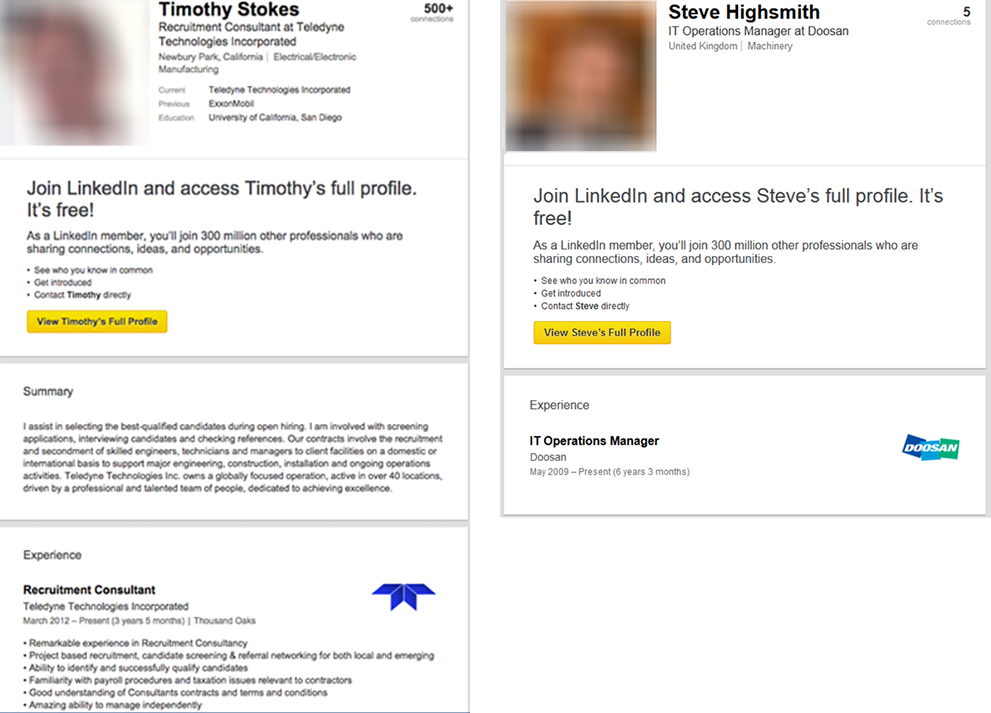
\includegraphics[width=0.6\textwidth]{Pic/linkedfake.png}
\end{center}

\end{frame}

\begin{frame}{Mia Ash \cite{mia_ash_lin}}

\begin{center}
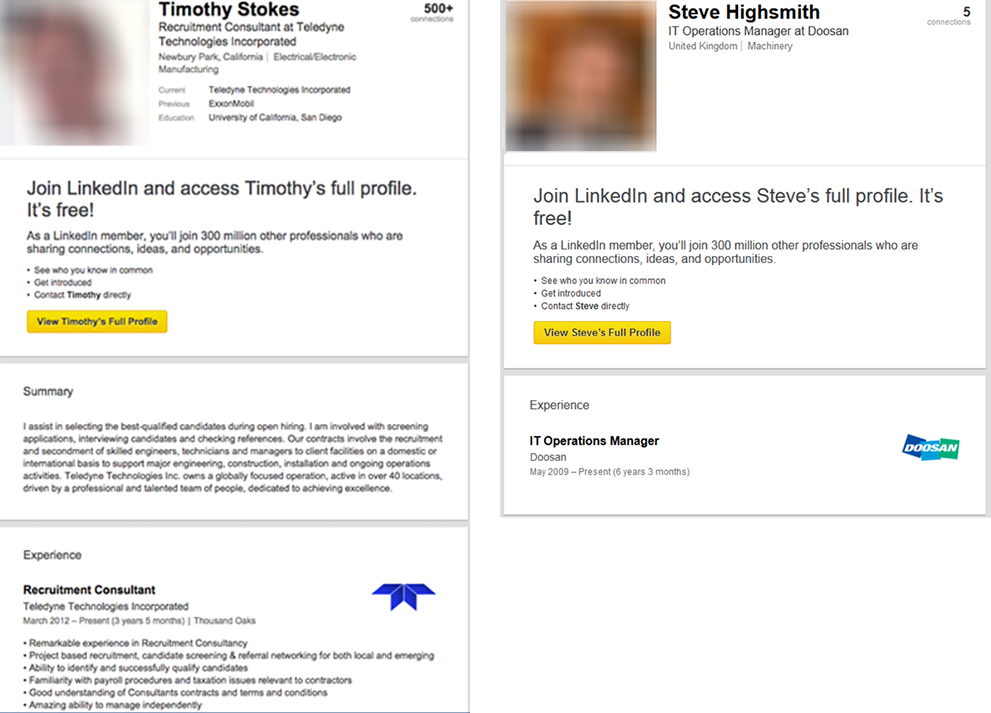
\includegraphics[width=0.6\textwidth]{Pic/linkedfake.png}
\end{center}

\end{frame}

\begin{frame}{Mia Ash \cite{mia_ash_lin}}

\begin{center}
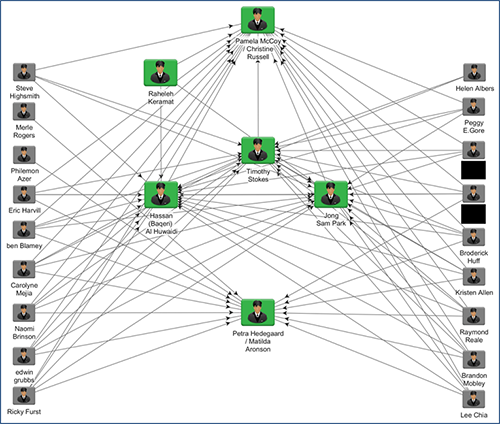
\includegraphics[width=0.6\textwidth]{Pic/linkedinnet.png}
\end{center}

\end{frame}

\begin{frame}{Mia Ash \cite{mia_ash_lin}}

\begin{center}
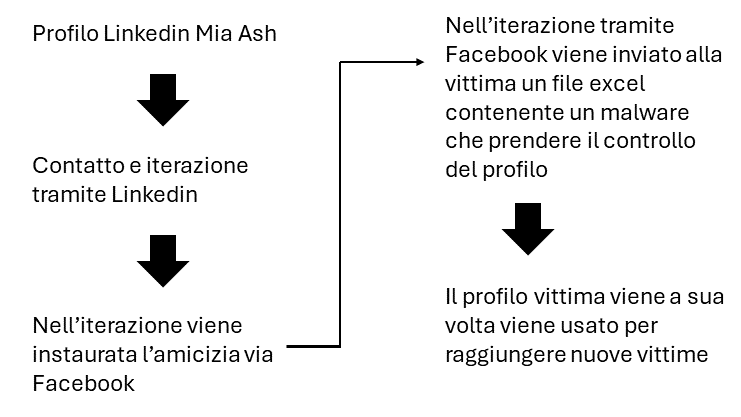
\includegraphics[width=0.6\textwidth]{Pic/MiaAsh_diagram.png}
\end{center}

\end{frame}

\begin{frame}{Mia Ash \cite{mia_ash_reuters}}

\begin{center}
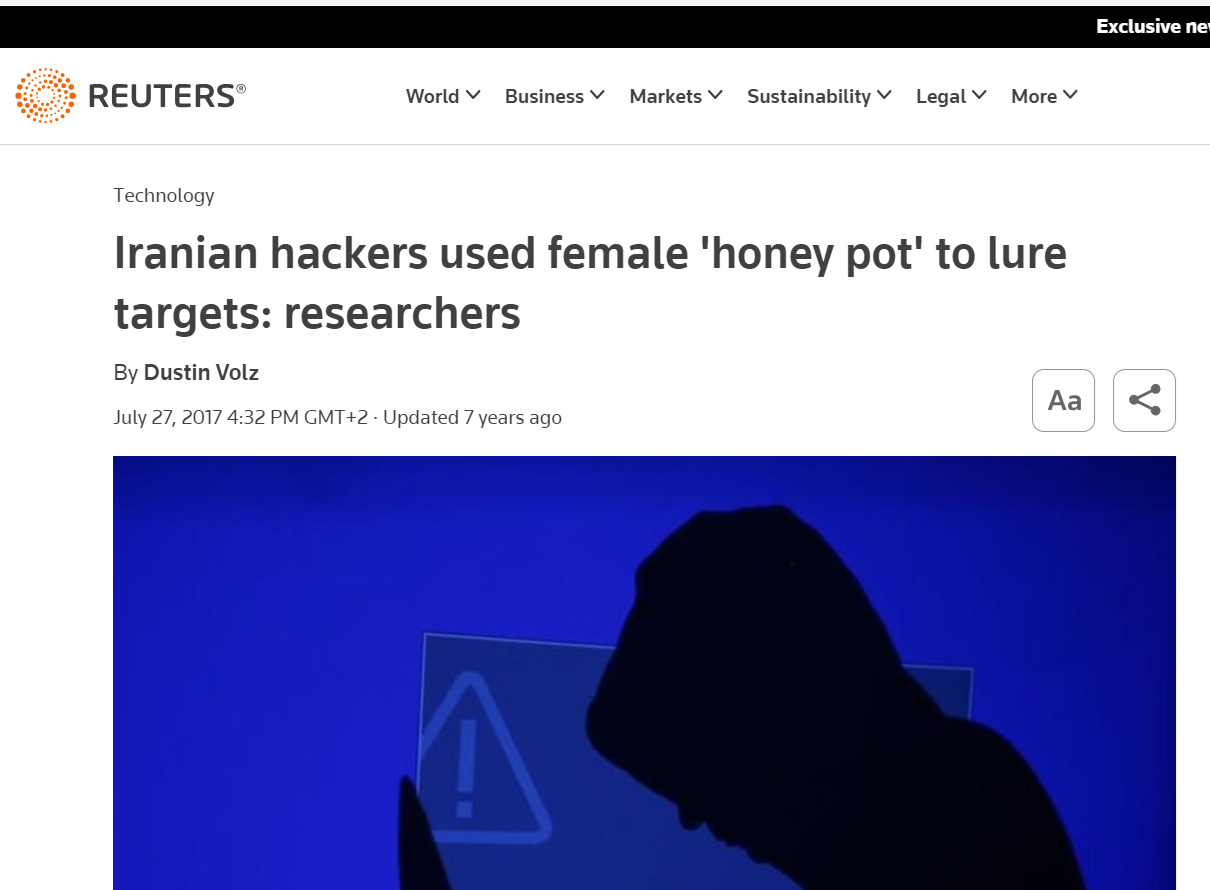
\includegraphics[width=0.8\textwidth]{Pic/reuters_miaash.png}
\end{center}

\end{frame}


\begin{frame}{IA generativa per il phishing \cite{genia_minacce}}

\begin{center}
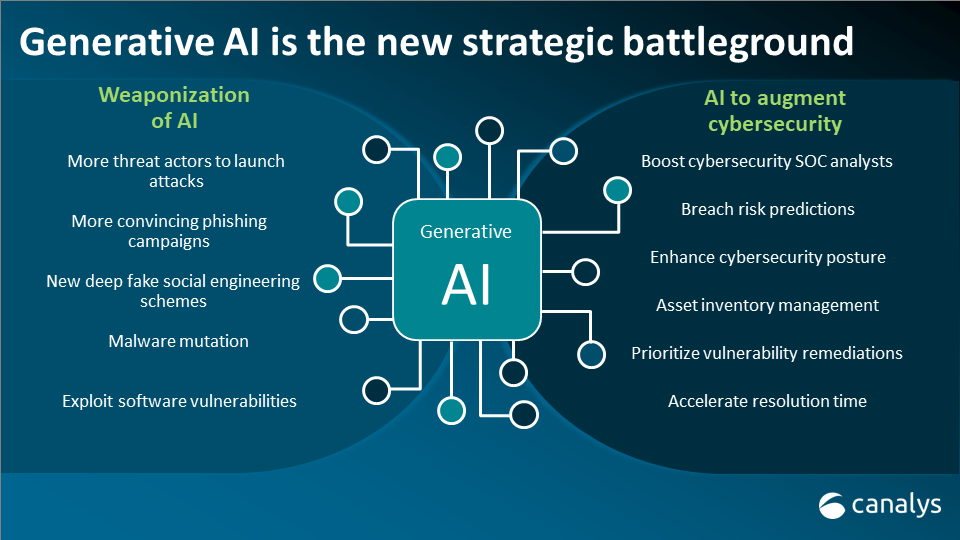
\includegraphics[width=0.8\textwidth]{Pic/GEN_IA_minacce.png}
\end{center}

\end{frame}

\begin{frame}{IA generativa per il phishing \cite{genia_gur}}

\begin{center}
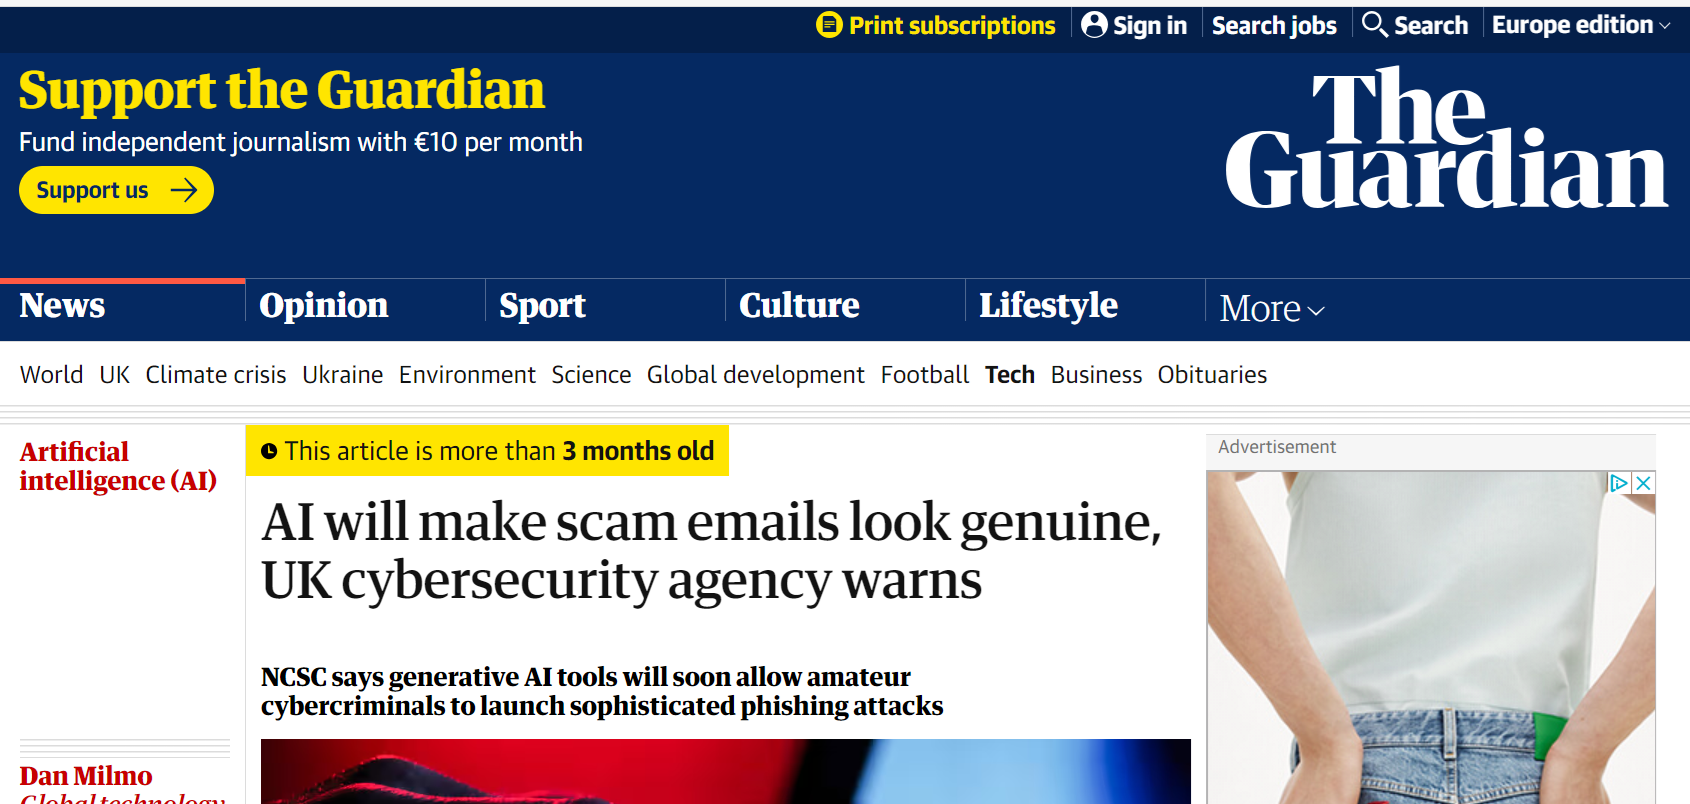
\includegraphics[width=0.8\textwidth]{Pic/AI_phishing.png}
\end{center}

\end{frame}

\begin{frame}{Click Farm \cite{clickfarm}}

\begin{center}
\includegraphics[width=0.8\textwidth]{Pic/cnn_click_farm.png}
\end{center}

\end{frame}



\begin{frame}{Click Farm }

\begin{center}

\includegraphics[width=0.8\textwidth]{Pic/compra_account_instagram.png}
\end{center}

\end{frame}

\begin{frame}{Click Farm }

\begin{center}
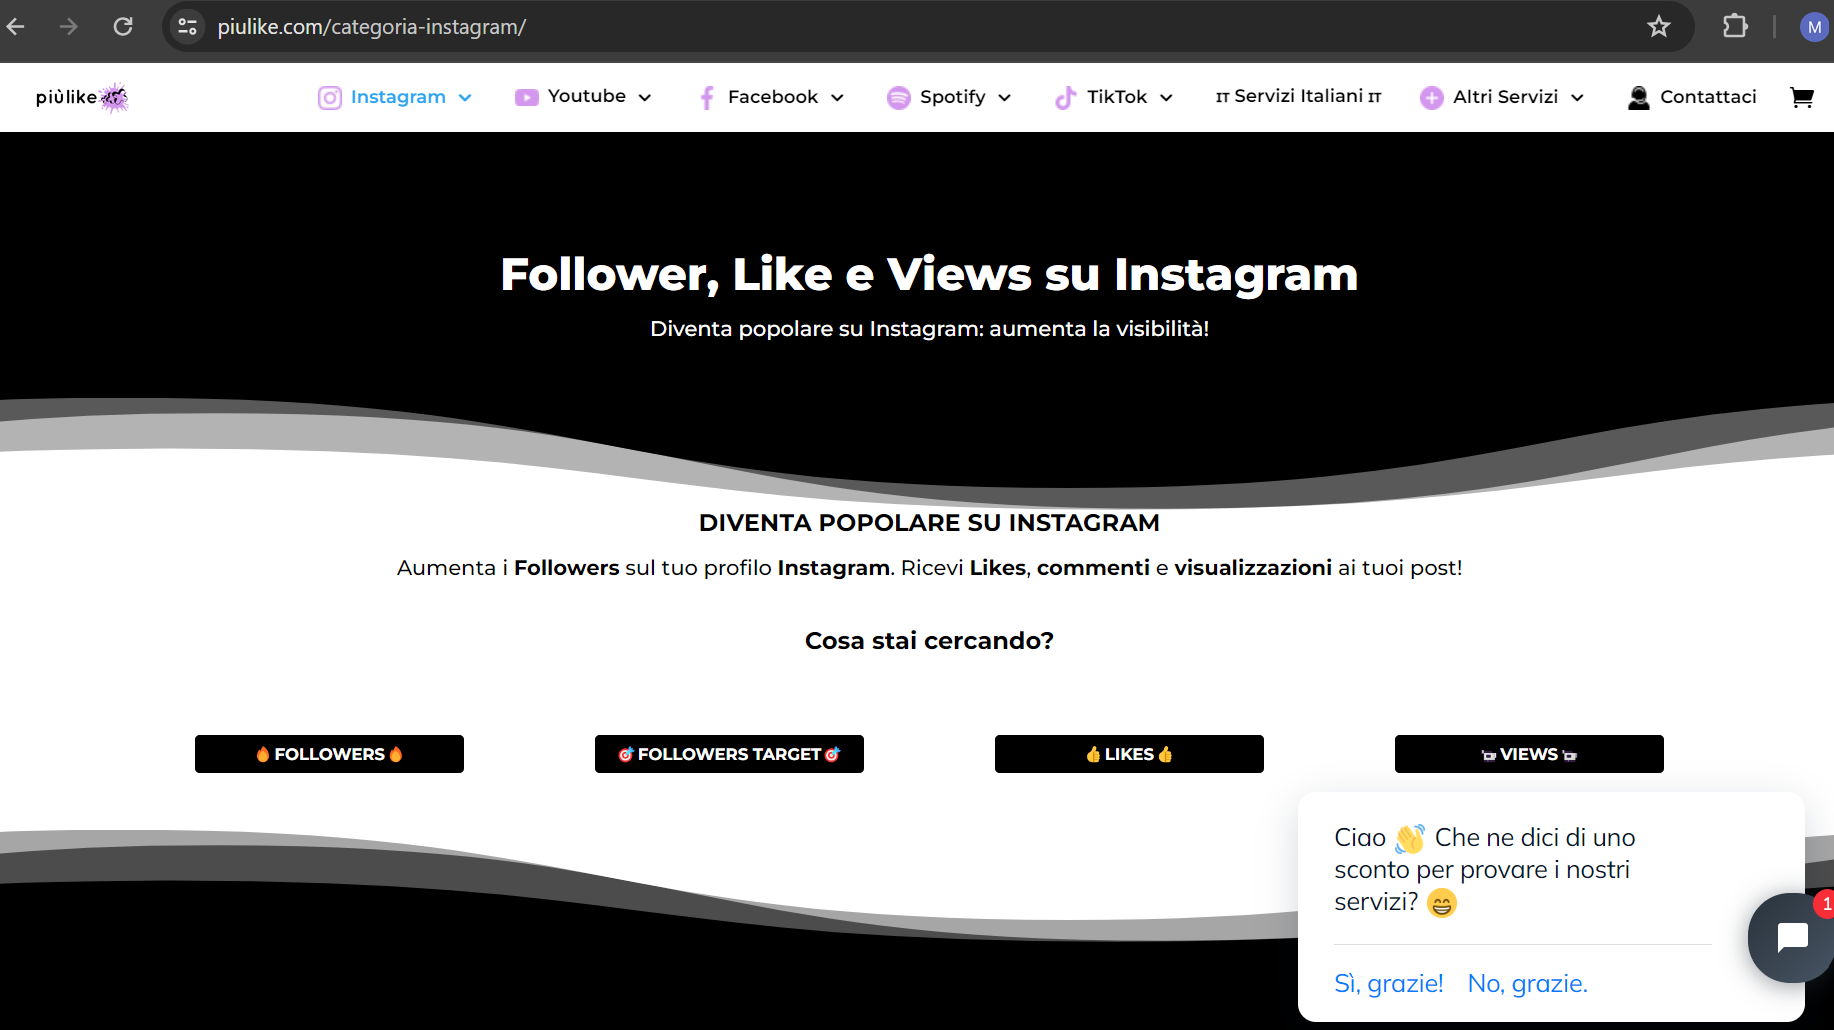
\includegraphics[width=0.8\textwidth]{Pic/compra_account_instagram_2.png}
\end{center}

\end{frame}

\begin{frame}{Click Farm \cite{social_nano}}

\begin{center}
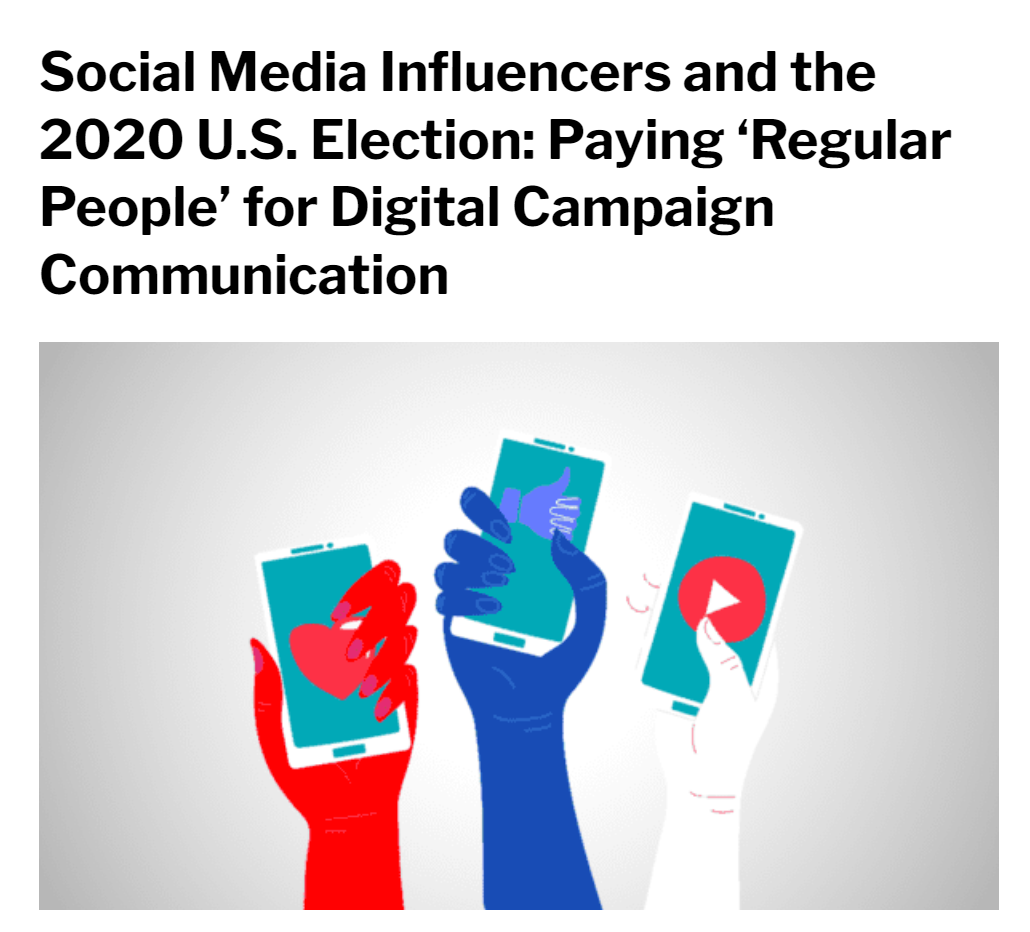
\includegraphics[width=0.6\textwidth]{Pic/nano_influence_politics.png}
\end{center}

\end{frame}


\begin{frame}{Manipolazione dei sistemi democratici}
\begin{alertblock}{Politica e nano-influencer  \cite{social_nano}}
"Coordinated networks of social media influencers, especially small-scale influencers with fewer than 10,000 followers, are now a powerful asset for political campaigns, PACs, and special interest groups. Partisan organizations are leveraging these “authentic” accounts in bids to sway political discourse and decision-making in the run up to the 2020 U.S. elections. Political marketers tell us that they see influencers, particularly those with more intimate followings, as regarded as more trustworthy by their followers and therefore better positioned to change their behavior"
\end{alertblock}
\end{frame}



\section{Definizioni}

\begin{frame}
\begin{center}
\Huge
Definizioni
\end{center}
\end{frame}

\begin{frame}{Deefake e Intelligenza Artificiale - definizioni}

\begin{alertblock}{Deepfake (NSA) \cite{nsa_definition}}
Contenuto multimediale creato sinteticamente o manipolato utilizzando una qualche forma di tecnologia meccanica o di deep learning.
\end{alertblock}

\begin{alertblock}{Intelligenza artificiale (NIST) \cite{nist_definitioN_AI}}
Una branca dell'informatica dedicata allo sviluppo di sistemi di elaborazione dati che svolgono funzioni normalmente associate all'intelligenza umana, come il ragionamento, l'apprendimento e l'auto-miglioramento
\end{alertblock}

\end{frame}

\begin{frame}{Deepfake e Intelligenza Artificiale - tassonomia \cite{tassonomia}}

\begin{center}
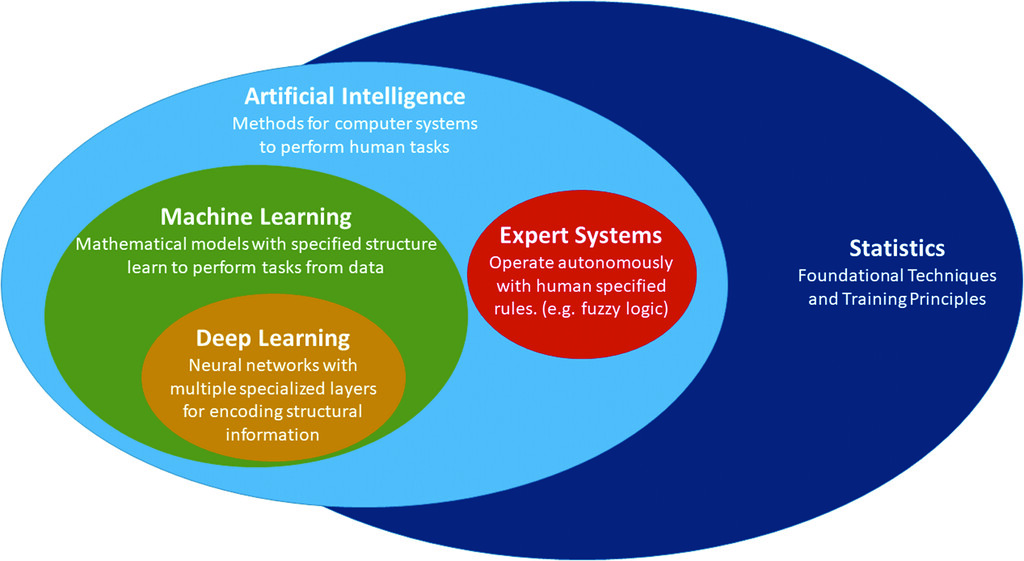
\includegraphics[width=0.8\textwidth]{Pic/IA_classification.jpg}
\end{center}

\end{frame}

\begin{frame}{Deepfake e Intelligenza Artificiale - reti neurali \cite{NN}}

\begin{center}
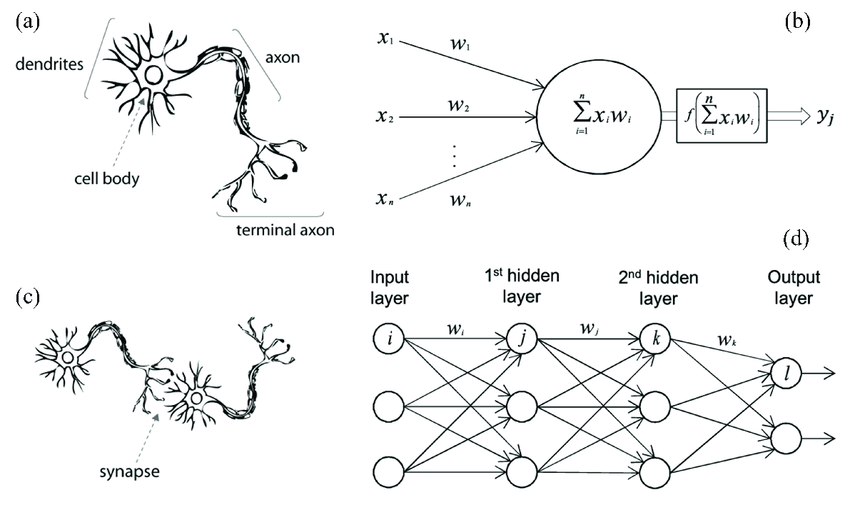
\includegraphics[width=0.8\textwidth]{Pic/Neural_network.png}
\end{center}

\end{frame}





\section{Breve storia}

\begin{frame}
\begin{center}
\Huge
Breve storia
\end{center}
\end{frame}

\begin{frame}{Storia dei deepfake }

\begin{center}
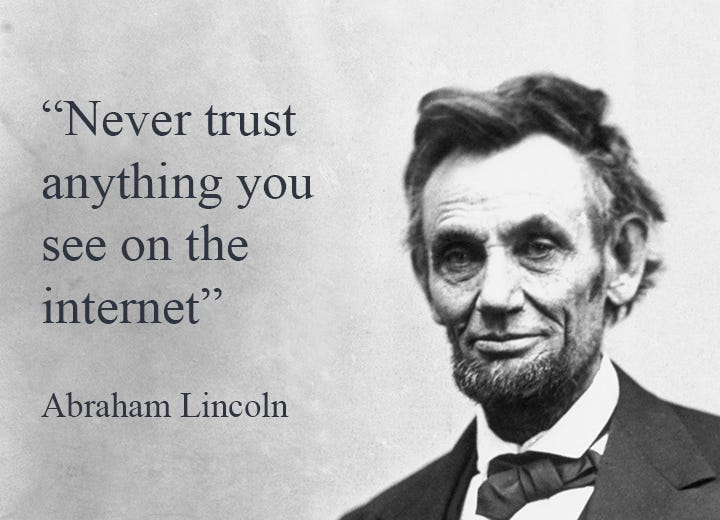
\includegraphics[width=0.8\textwidth]{Pic/lincon.jpg}
\end{center}

\end{frame}


\begin{frame}{Storia dei deepfake: 1860 Calhoun/Lincon \cite{ng}}

\begin{center}
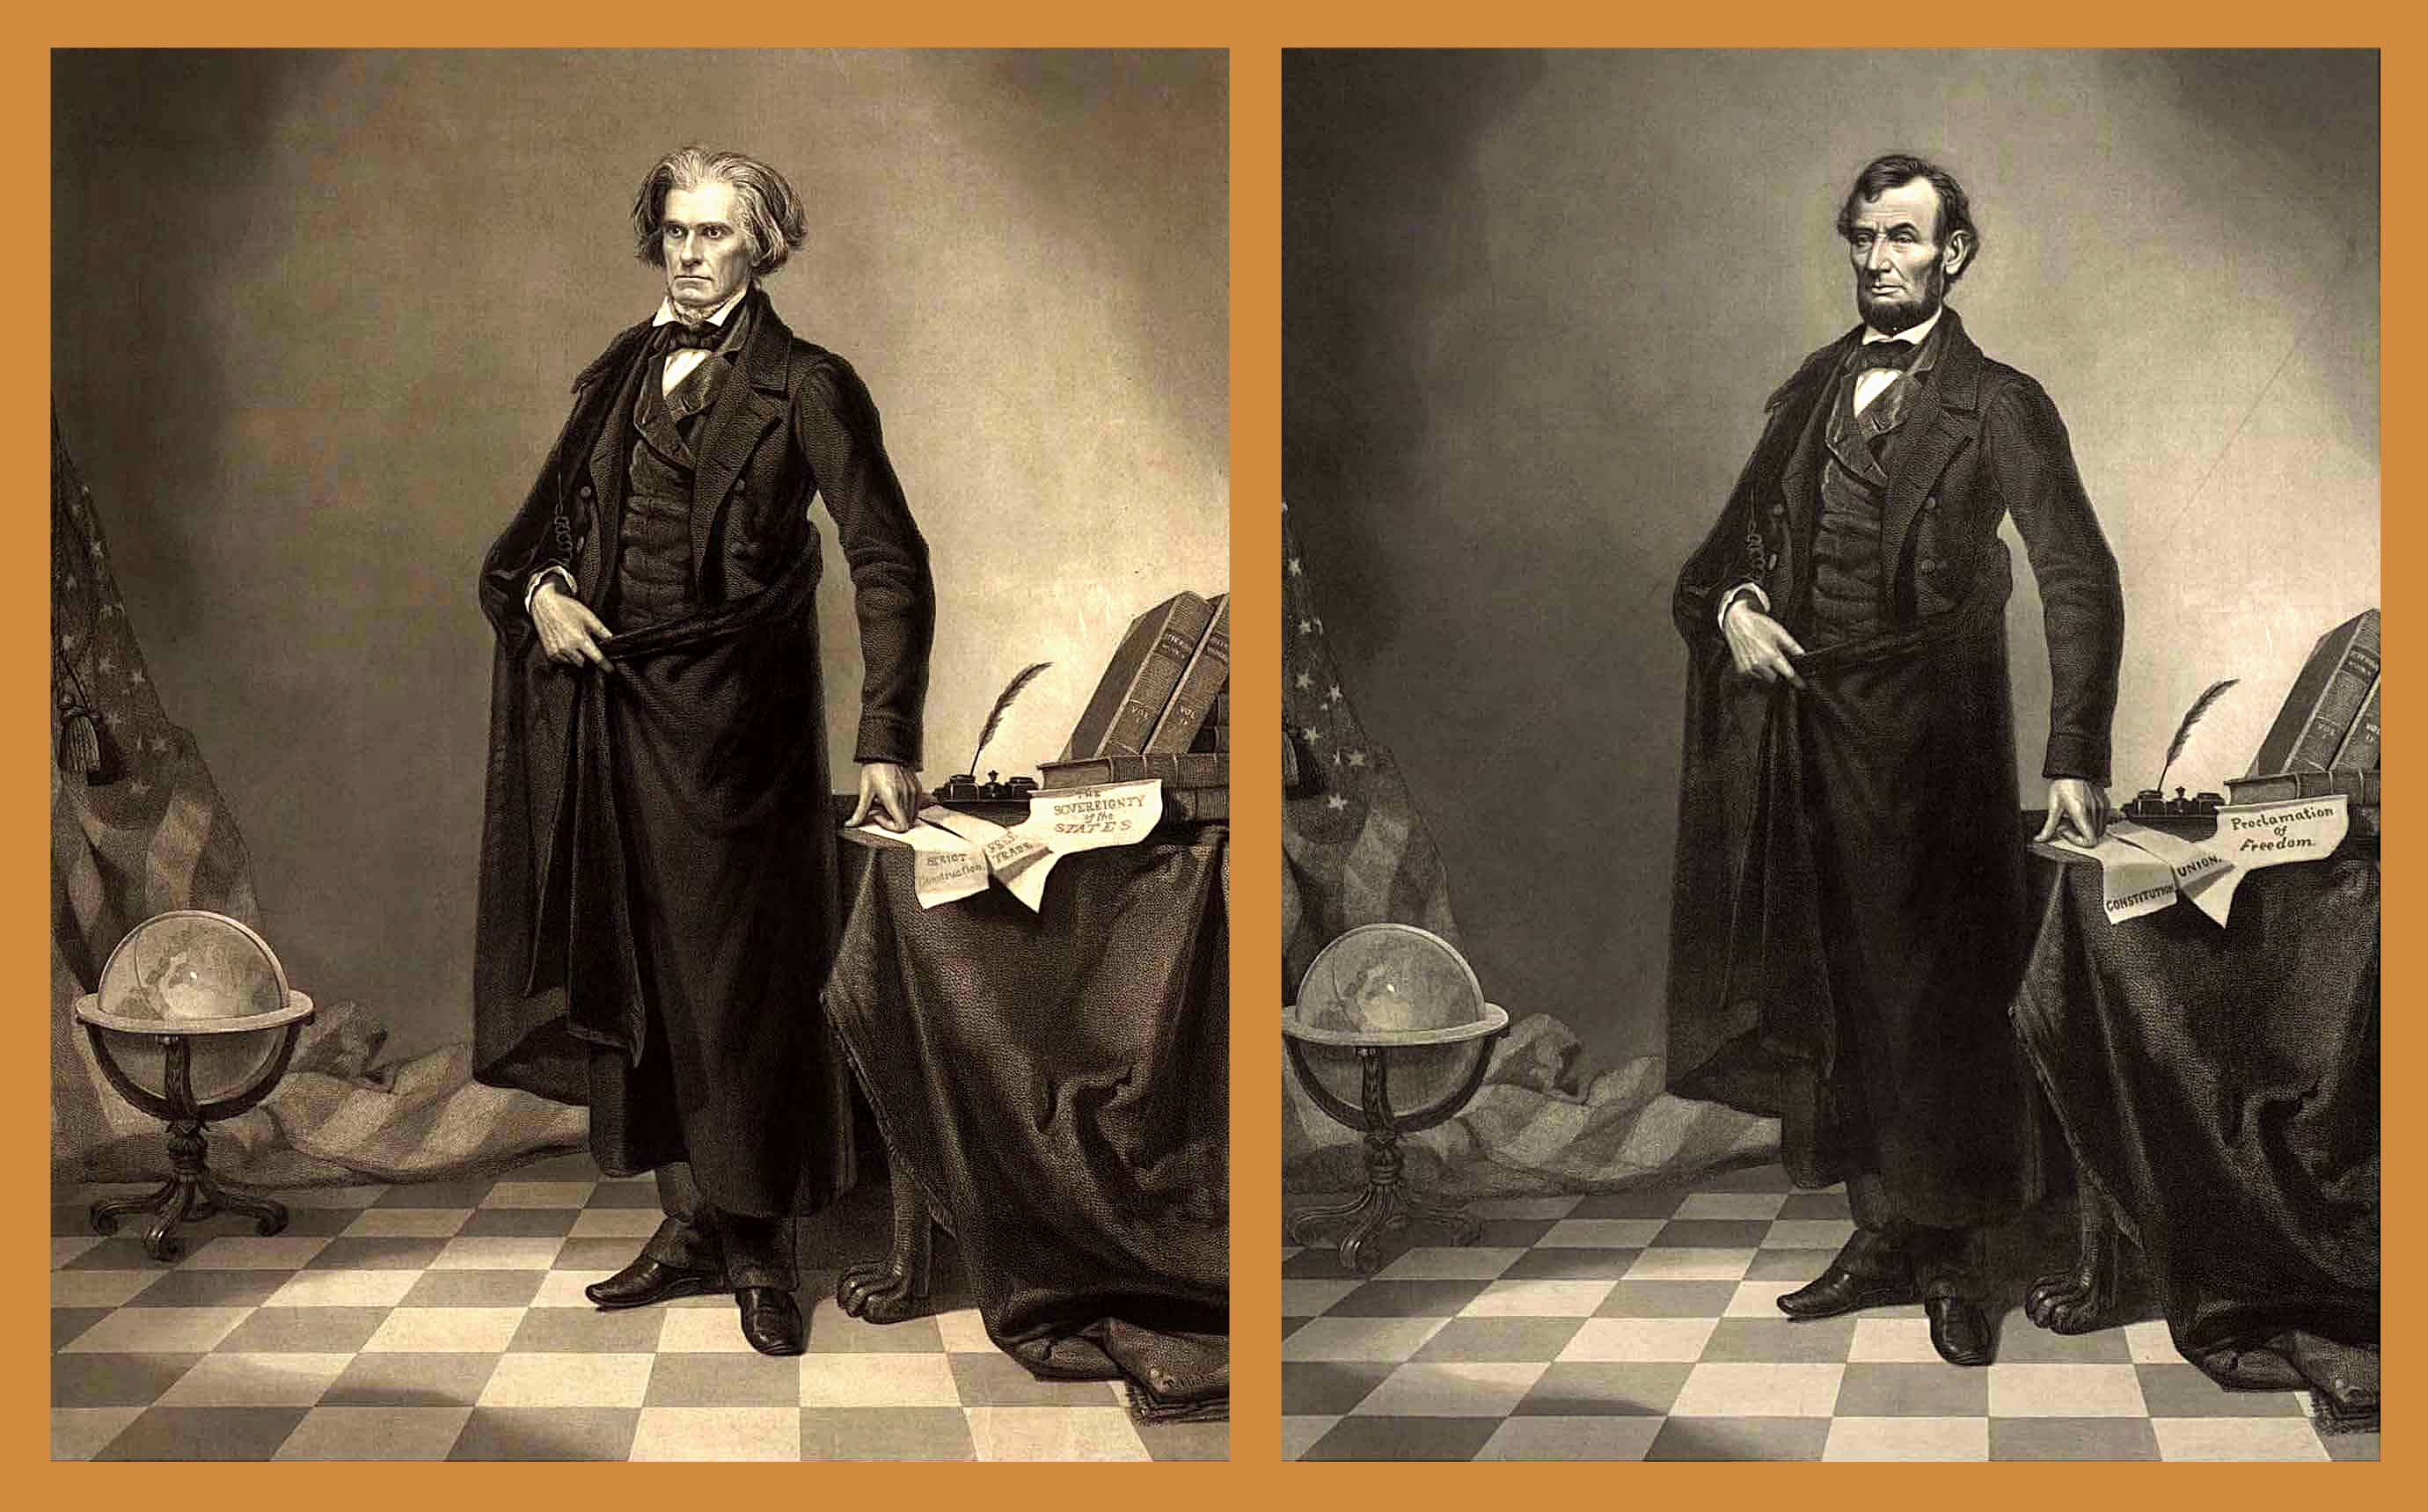
\includegraphics[width=0.8\textwidth]{Pic/Licon_deepfake.jpg}
\end{center}

\end{frame}


\begin{frame}{Storia dei deepfake: 1997 Video Rewrite (GAN) \cite{video_rewrite}}

\begin{center}
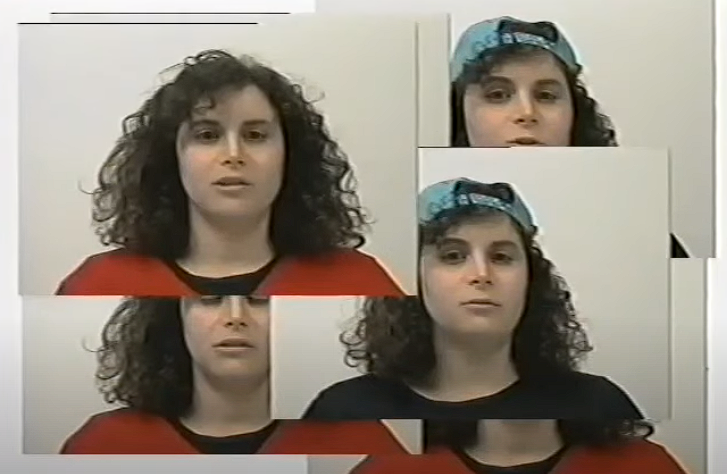
\includegraphics[width=0.8\textwidth]{Pic/video_rewrite.png}
\end{center}

\end{frame}


\begin{frame}{Deepfake e Intelligenza Artificiale - tassonomia \cite{masood2023deepfakes}}

\begin{center}
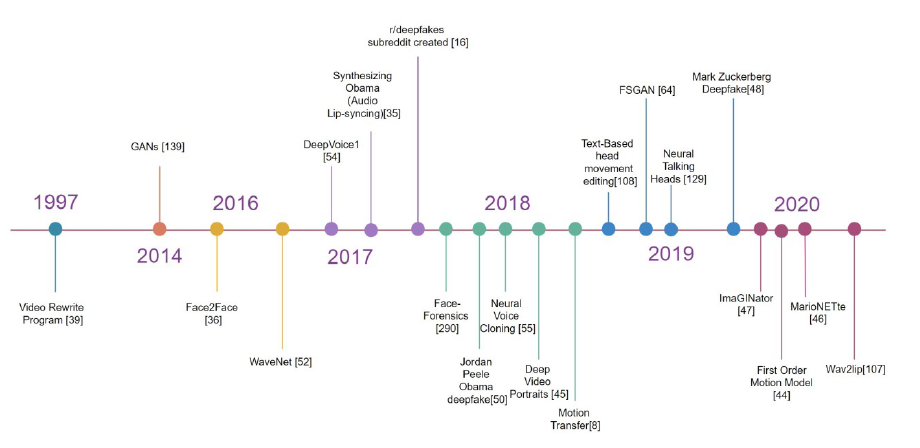
\includegraphics[width=0.8\textwidth]{Pic/timeline_deepfakes.png}
\end{center}

\end{frame}


\begin{frame}{Storia dei deepfake: 2017 B.Obama \cite{reuters_fake}}

\begin{center}
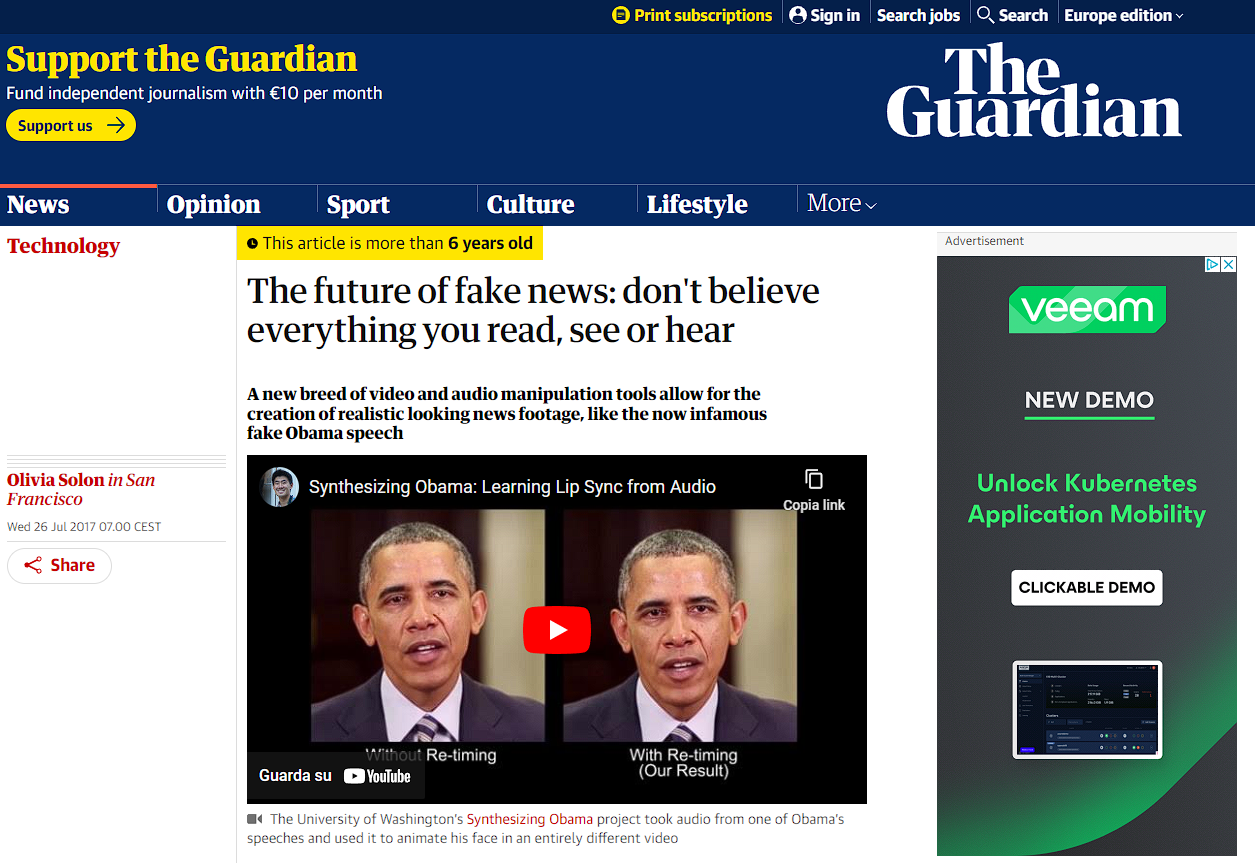
\includegraphics[width=0.8\textwidth]{Pic/guardian_obama.png}
\end{center}

\end{frame}

\begin{frame}{Storia dei deepfake: 2017 Imitazione della voce \cite{wsj_audio}}

\begin{center}
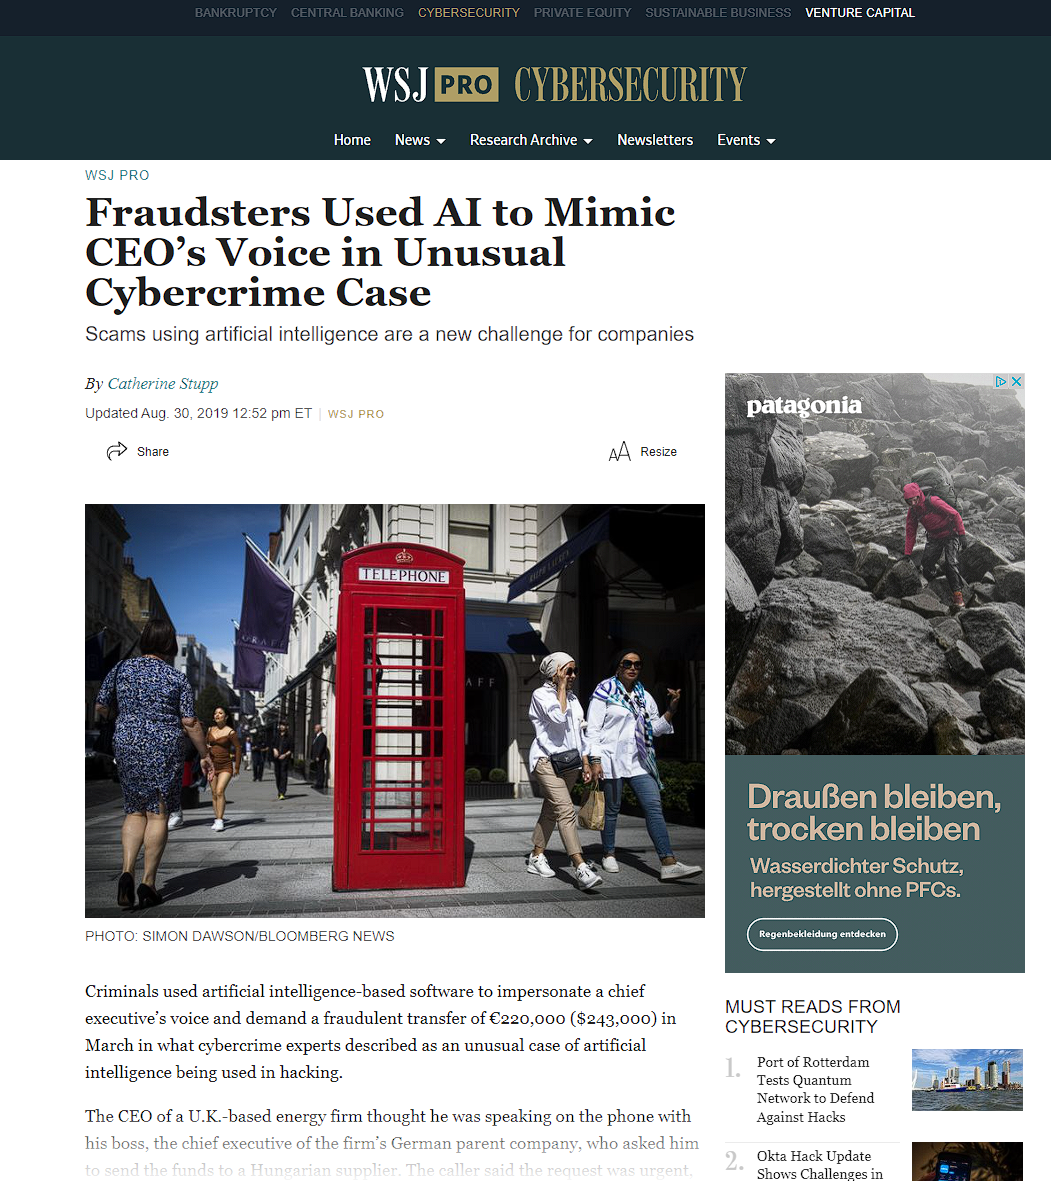
\includegraphics[width=0.6\textwidth]{Pic/deepfake_audio.png}
\end{center}

\end{frame}




\begin{frame}{Storia dei deepfake: 2020 N.Pelosi \cite{wsj_audio}}

\begin{center}
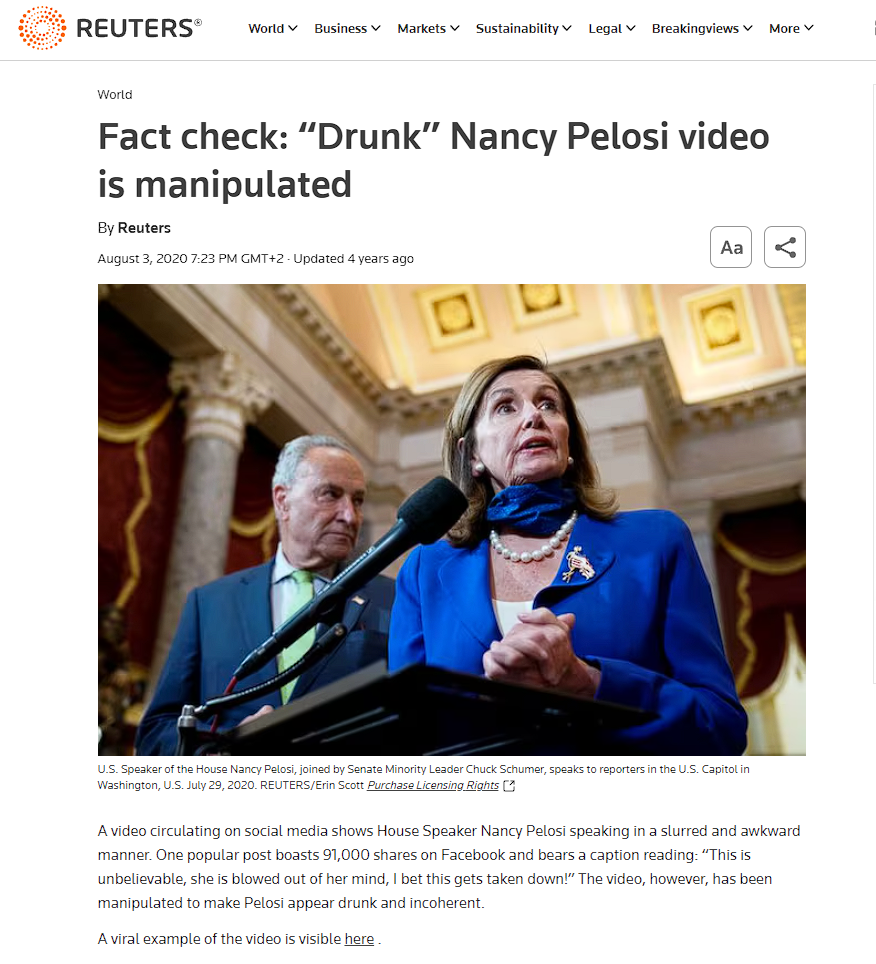
\includegraphics[width=0.6\textwidth]{Pic/fake_video_pelosi.png}
\end{center}

\end{frame}

\begin{frame}{Storia dei deepfake: Software disponibili \cite{masood2023deepfakes}}

\begin{center}
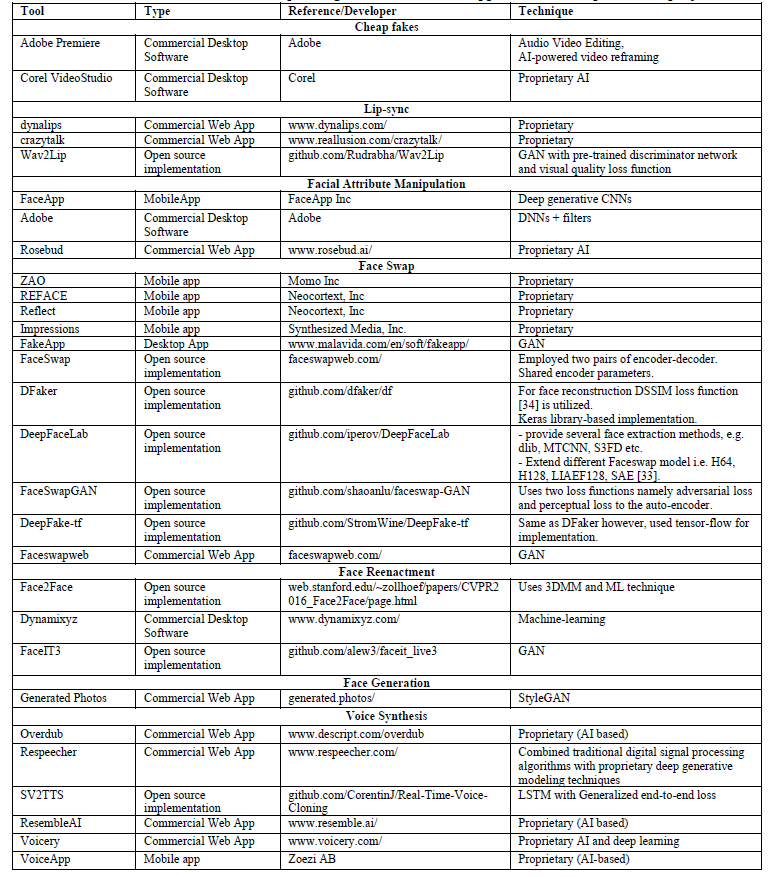
\includegraphics[width=0.5\textwidth]{Pic/deepfake_tools.png}
\end{center}

\end{frame}


\section{Fondamenti teorici/computazionali}

\begin{frame}
\begin{center}
\Huge
Fondamenti teorici/computazionali
\end{center}
\end{frame}


\begin{frame}{Machine learning \cite{pml1Book,pml2Book,classification_datacamp}}

\begin{alertblock}{Distribuzione di probabilità condizionata - idea }
Abbiamo una serie di record che contengono delle variabili  input (dimensione del fiore, colore etc..) e una variabile di output (caso semplice, può essere generalizzato). Non sappiamo a priori come input e output siano legati (altrimenti avremmo risolto il problema !), ma siamo interessati a trovare una funzione di probabilità che associ degli input a degli output. $p(y=c|\textbf{x};\bm{\theta})=f_{c}(\textbf{x};\bm{\theta})$
\end{alertblock}


\end{frame}

\begin{frame}{Machine learning \cite{pml1Book,pml2Book,classification_datacamp}}
\begin{center}
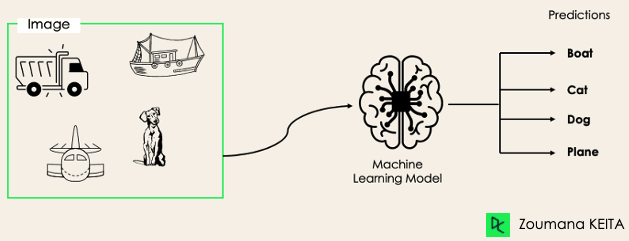
\includegraphics[width=0.8\textwidth]{Pic/4_label_classification_task_Datacamp.png}
\end{center}


\end{frame}



\begin{frame}{Machine learning \cite{pml1Book,pml2Book,classification,regression}}


\begin{columns}
\begin{column}{0.5\textwidth}
\begin{center}
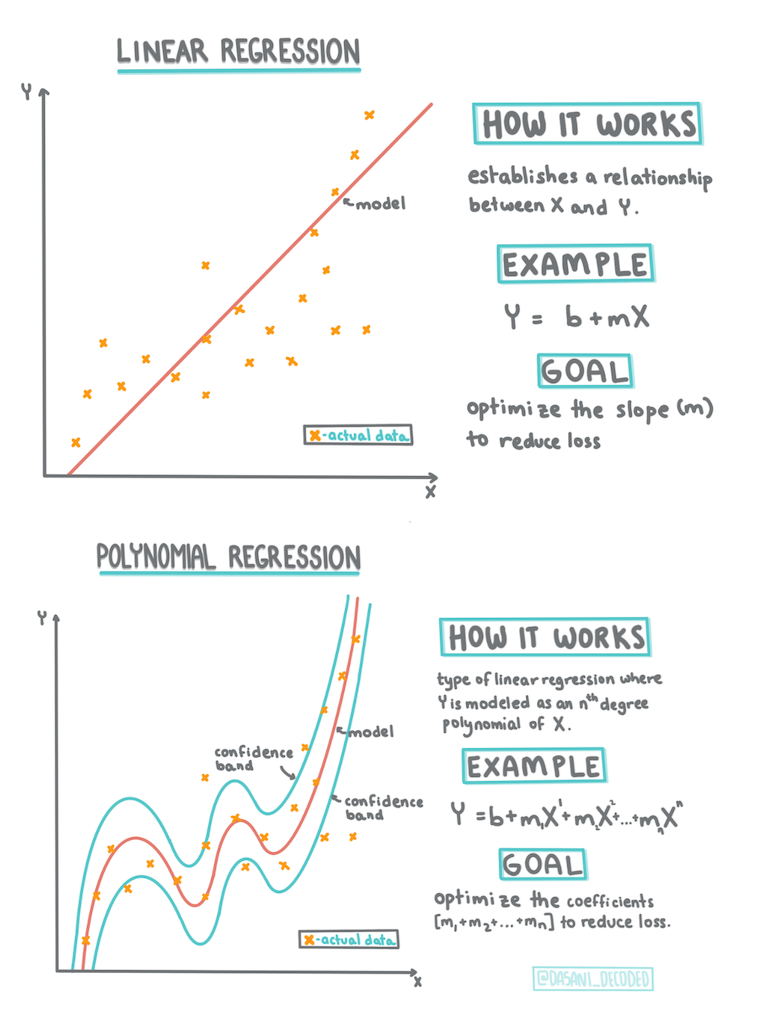
\includegraphics[width=0.8\textwidth]{Pic/regression.png}
\end{center}
\end{column}
\begin{column}{0.4\textwidth}  
\begin{center}
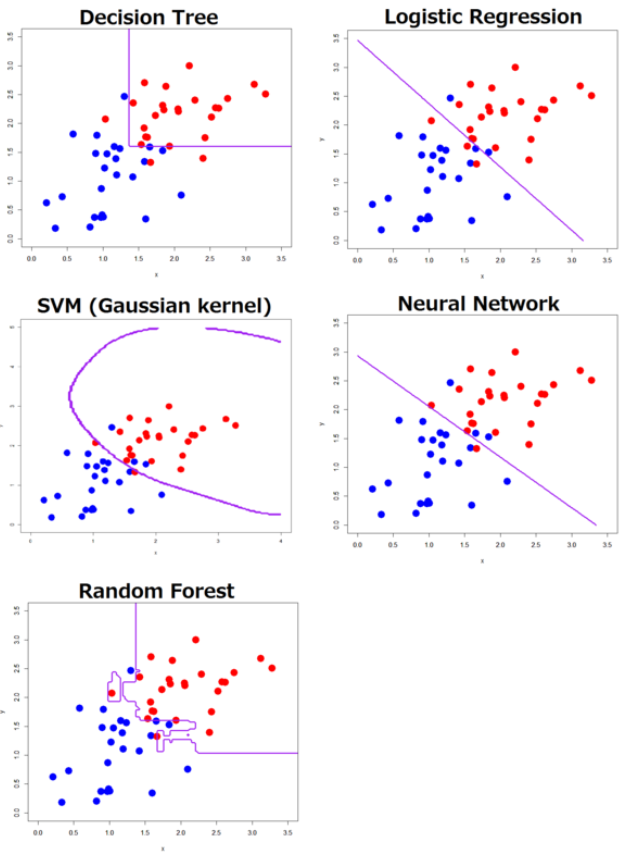
\includegraphics[width=0.6\textwidth]{Pic/classification.png}
\end{center}
\begin{alertblock}{No free lunch theorem}
Non esiste un modello che abbia performance migliori in tutti i casi possibili. Ciò è dovuto al fatto che ogni modello fa delle assunzioni.
\end{alertblock}
\end{column}
\end{columns}
\end{frame}

\begin{frame}{Machine learning \cite{pml1Book,pml2Book,classification,regression,bd}}

\begin{center}
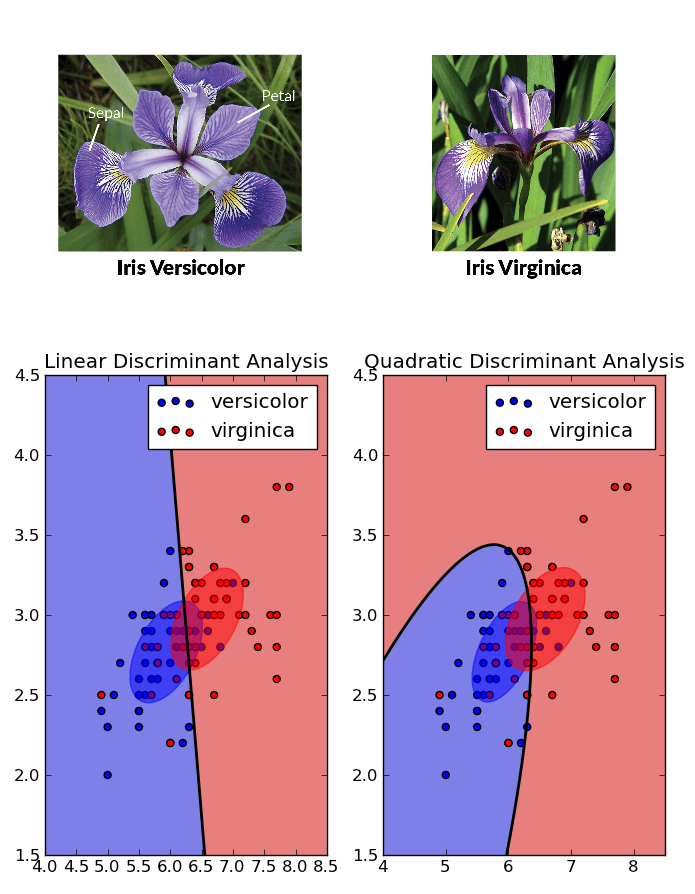
\includegraphics[width=0.5\textwidth]{Pic/decision_boundary_example.png}
\end{center}


\end{frame}



\begin{frame}{Machine learning \cite{pml1Book,pml2Book,classification,regression,KirkDBorne}}

\begin{center}
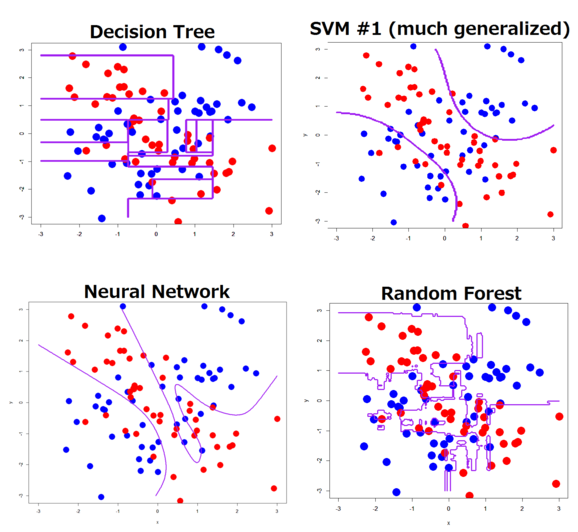
\includegraphics[width=0.5\textwidth]{Pic/ML_dec_boundary.png}
\end{center}


\end{frame}




\begin{frame}{Reti neurali \cite{pml1Book,pml2Book}}
\begin{center}
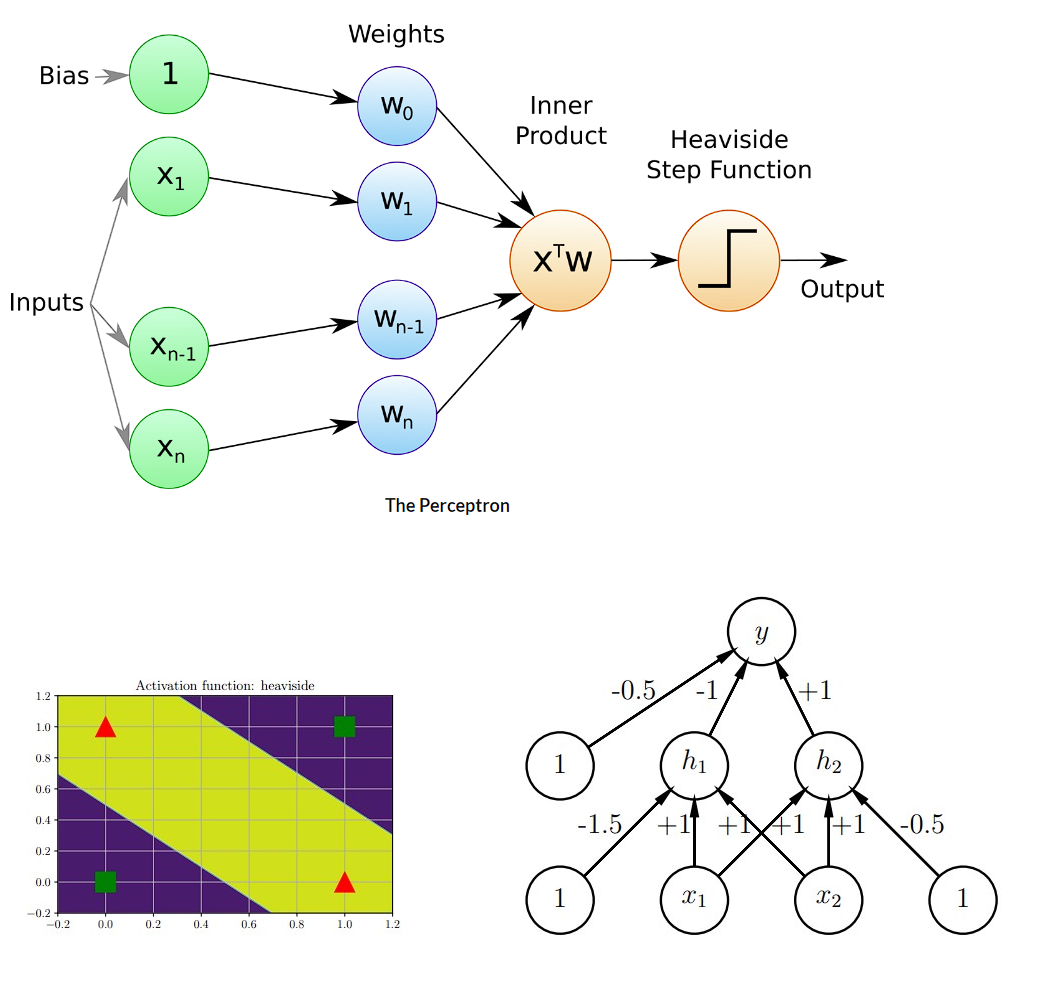
\includegraphics[width=0.7\textwidth]{Pic/perceptron.png}
\end{center}
\end{frame}



\begin{frame}{Modelli generativi \cite{google_generativeIA,pml1Book,pml2Book}}
\begin{columns}
\begin{column}{0.5\textwidth}
\begin{alertblock}{Modello generativo}
Un modello generativo descrive come viene generato un set di dati utilizzando un modello probabilistico $(p(x)\quad x\in X)$. Campionando da questo modello, siamo in grado di generare nuovi dati.
\end{alertblock}
\begin{center}
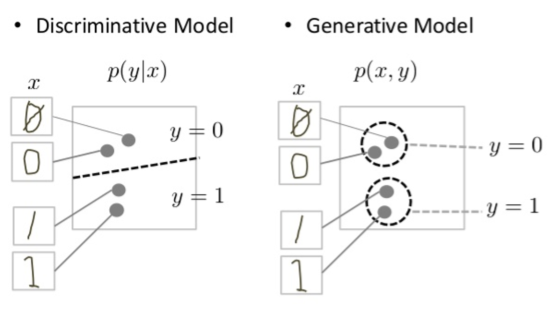
\includegraphics[width=\textwidth]{Pic/generative_v_discriminative.png}
\end{center}
\end{column}
\begin{column}{0.4\textwidth}  
\begin{alertblock}{Tipologia di modelli generativi}
\begin{itemize}
\item Deep generative models (DGM): viene usata una deep neural network. Comprende i Variational Autoencoder (VAE) e le Generative adversarial network oltre che, ad esempio, i Diffusion models e gli Energy based models (EBM)
\item Probabilistic graphical models: viene usato un grafo causale 
\end{itemize}
\end{alertblock}
\end{column}
\end{columns}
\end{frame}

\begin{frame}{Modelli generativi \cite{pml1Book,pml2Book}}
\begin{center}
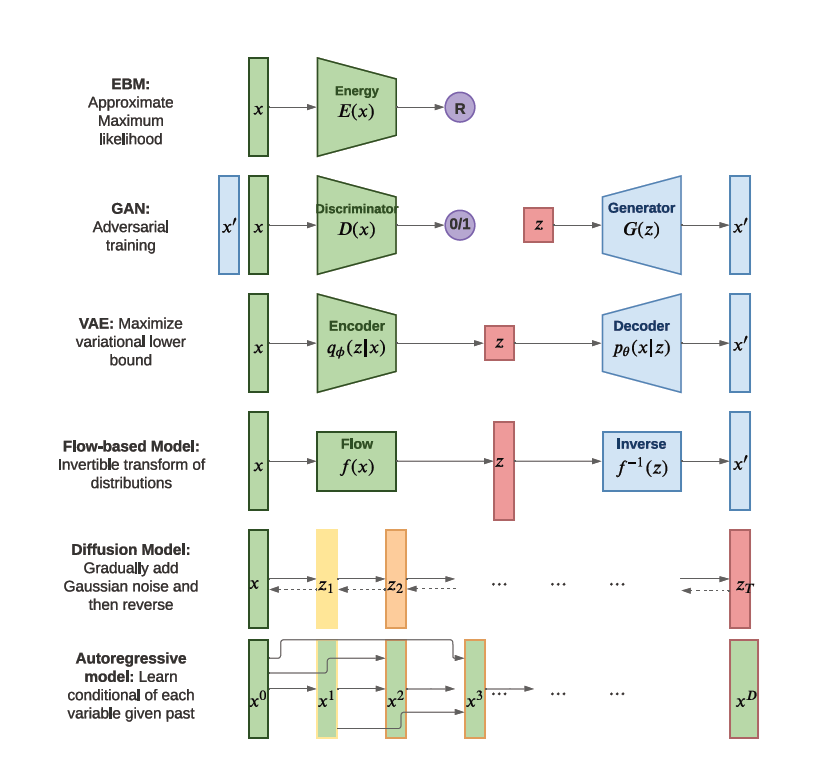
\includegraphics[width=0.7\textwidth]{Pic/generative_models.png}
\end{center}
\end{frame}

\begin{frame}{Autoencoders: esempi \cite{pml1Book,pml2Book,autoencoder_comp}}
\begin{center}
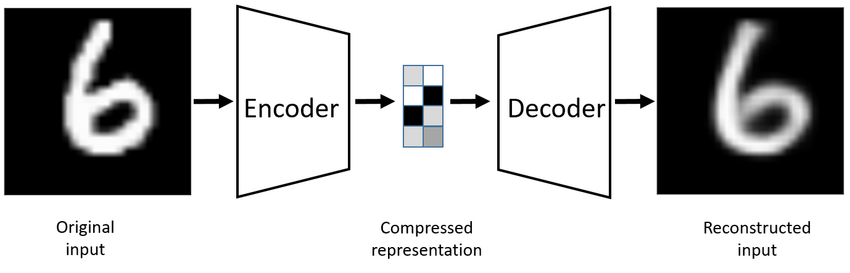
\includegraphics[width=0.8\textwidth]{Pic/CompressionVAE.png}
\end{center}
\end{frame}


\begin{frame}{Autoencoders \cite{pml1Book,pml2Book}}
\begin{columns}
\begin{column}{0.5\textwidth}
\begin{alertblock}{Autoencoder}
Encoder ($f_{e}$) +   Decoder $f_{d}$ \\
$f_{e}: x \rightarrow z$ $f_{d}: z \rightarrow x$ \\ $ r(x)= f_{d}(f_{e}(x))$ (rec. function )\\$\mathcal{L}(\theta)=||r(x)-x||^{2}$ (loss function)
\end{alertblock}
\begin{alertblock}{Funzionamento}
L'unità in mezzo agisce come collo di bottiglia tra l'input e la sua ricostruzione, in modo da applicare una compressione.
\end{alertblock}
\end{column}
\begin{column}{0.4\textwidth}  
\begin{center}
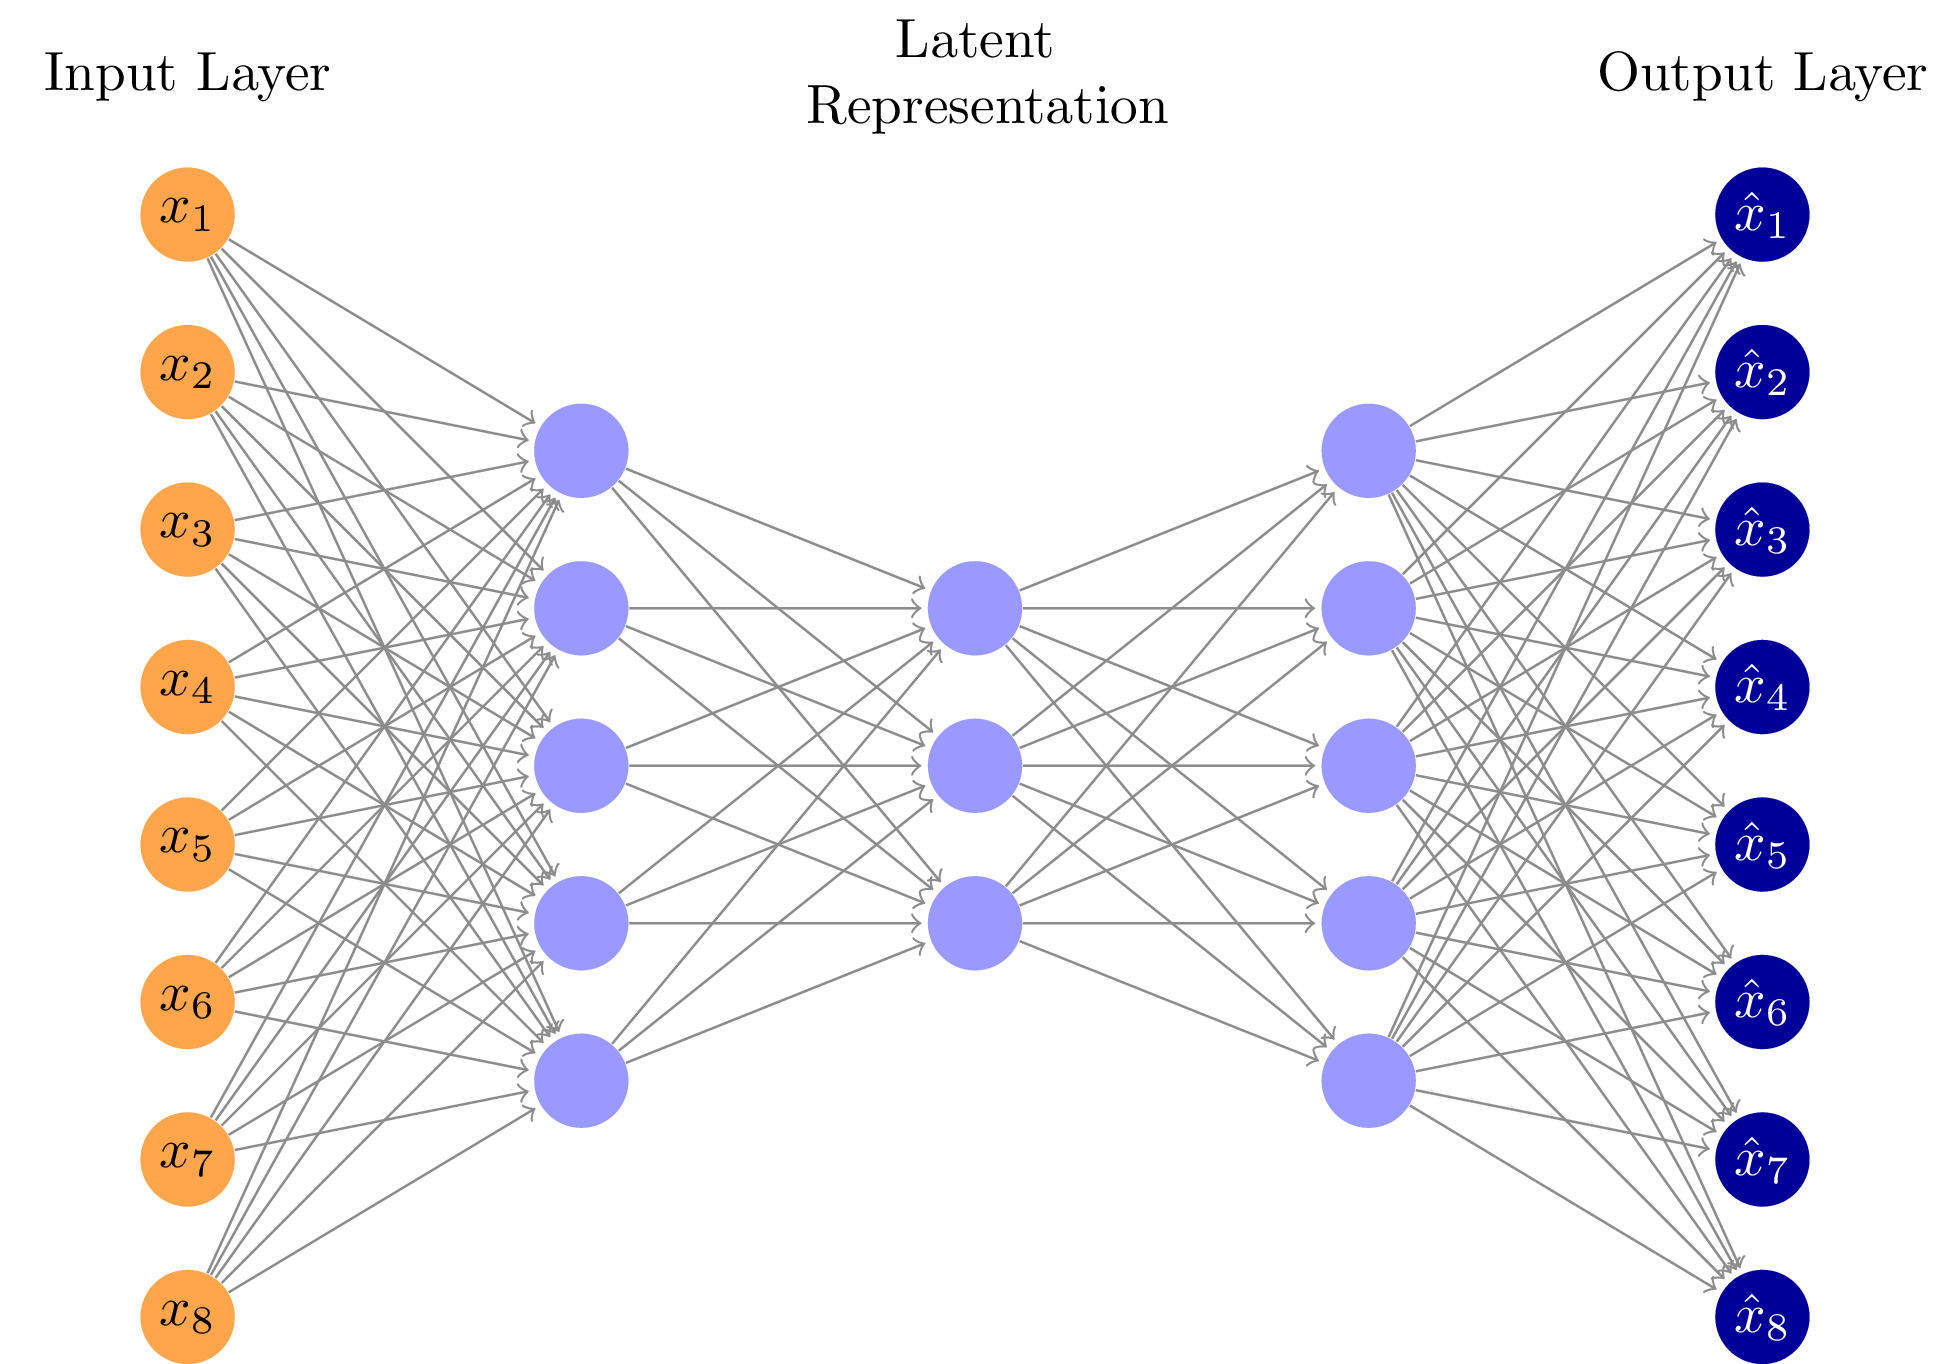
\includegraphics[width=\textwidth]{Pic/autoencoder.png}
\end{center}
\end{column}
\end{columns}
\end{frame}

\begin{frame}{Autoencoders \cite{pml1Book}}
\begin{center}
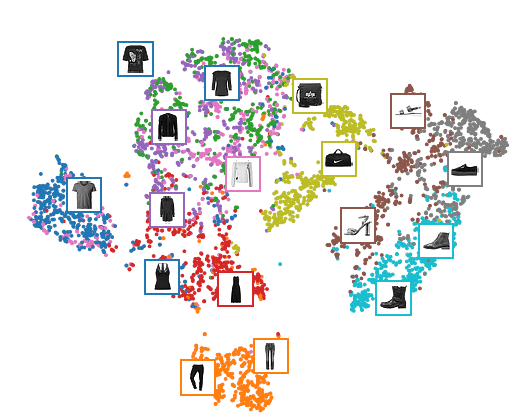
\includegraphics[width=0.8\textwidth]{Pic/autoencoder_ex.png}
\end{center}
\end{frame}


\begin{frame}{Variational autoencoders \cite{pml1Book,pml2Book}}
\begin{columns}
\begin{column}{0.5\textwidth}
\begin{alertblock}{Modello generativo}
Un modello generativo descrive come viene generato un set di dati utilizzando un modello probabilistico $(p(x)\quad x\in X)$. Campionando da questo modello, siamo in grado di generare nuovi dati.
\end{alertblock}
\begin{alertblock}{Differenza rispetto agli AE}
Rispetto agli autoencoder i variational autoencoder possono essere visti come una versione probabilistica di un autoencoder deterministico. In questo modo si può avere una IA generativa
\end{alertblock}
\end{column}
\begin{column}{0.4\textwidth}  
\begin{center}
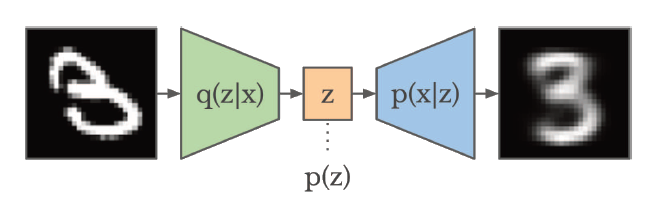
\includegraphics[width=\textwidth]{Pic/variational_auto_diag.png}
\end{center}
\begin{alertblock}{Remark}
La VAE, per come è costruita, è in grado di convertire punti casuali in output, mentre il decoder di AE (deterministico) funziona solo per un punto che è già presente nel training. 
\end{alertblock}
\begin{center}
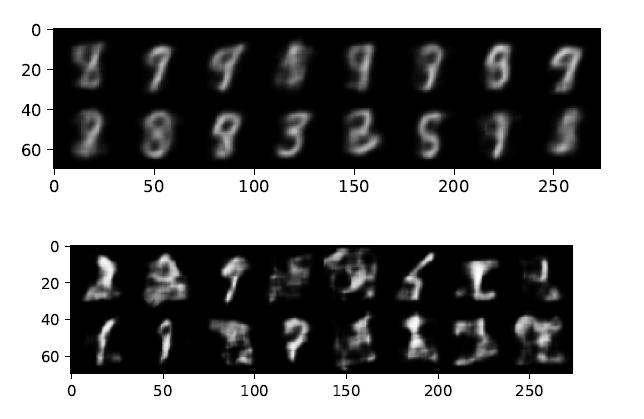
\includegraphics[width=0.3\textwidth]{Pic/AE_vs_VAE.png}
\end{center}
\end{column}
\end{columns}
\end{frame}

\begin{frame}{VAR generation \cite{pml1Book,pml2Book}}
\begin{center}
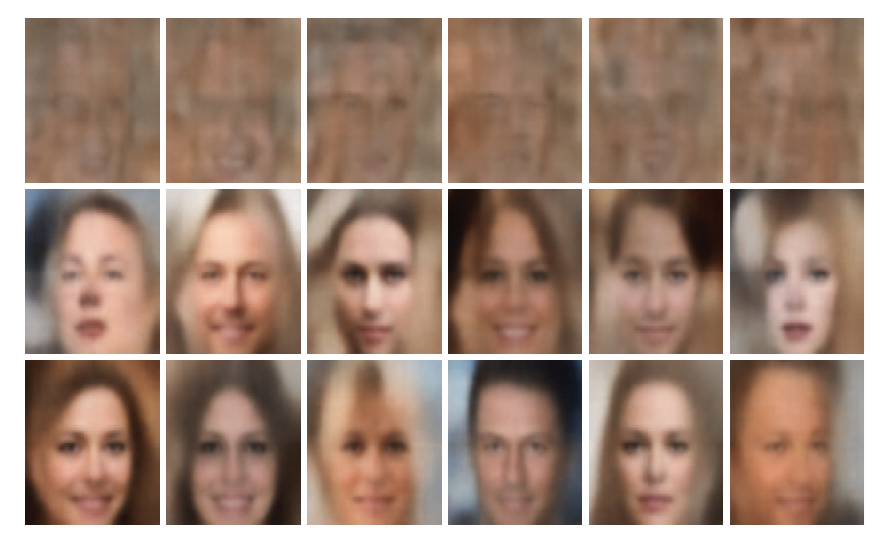
\includegraphics[width=0.8\textwidth]{Pic/var_generation.png}
\end{center}
\end{frame}

\begin{frame}{Generative adversarial networks \cite{pml1Book,pml2Book}}
\begin{columns}
\begin{column}{0.5\textwidth}
\begin{alertblock}{Idea}
Ho due reti neurali
\begin{itemize}
\item Generatore: creare nuovi dati
\item Discriminatore: distinguere i dati nuovi da quelli veri
\end{itemize}
\end{alertblock}
\end{column}
\begin{column}{0.4\textwidth}  
\begin{center}

\includegraphics[width=\textwidth]{Pic/GAN.png}
\end{center}
\begin{center}
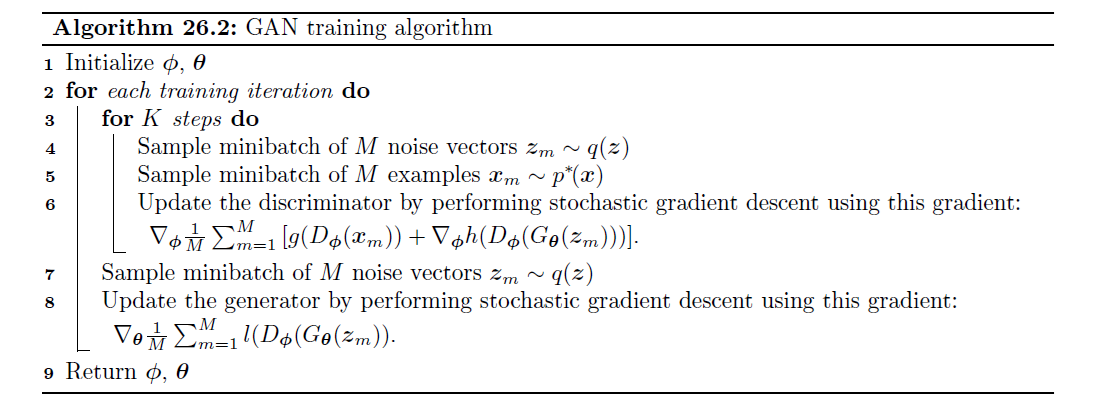
\includegraphics[width=\textwidth]{Pic/algorithm_GAN.png}
\end{center}
\end{column}
\end{columns}
\end{frame}


\begin{frame}{VAR generation \cite{nguyen2017plug}}
\begin{center}
\includegraphics[width=0.6\textwidth]{Pic/GAN_example.png}
\end{center}
\end{frame}


\section{Difesa: come rilevarle ?}

\begin{frame}
\begin{center}
\Huge
Difesa: come rilevarle ?
\end{center}
\end{frame}

\begin{frame}{Metodi \cite{masood2023deepfakes}}
\begin{center}
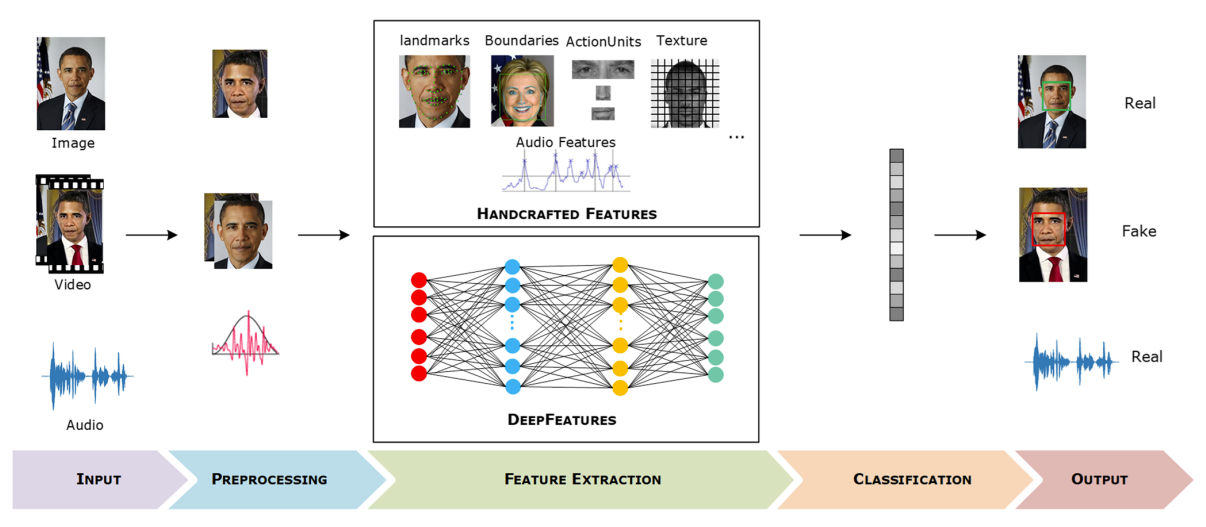
\includegraphics[width=0.8\textwidth]{Pic/deepfake_detection.png}
\end{center}
\end{frame}


\begin{frame}{Error level analysis \cite{jeronymo2017image}}
\begin{center}
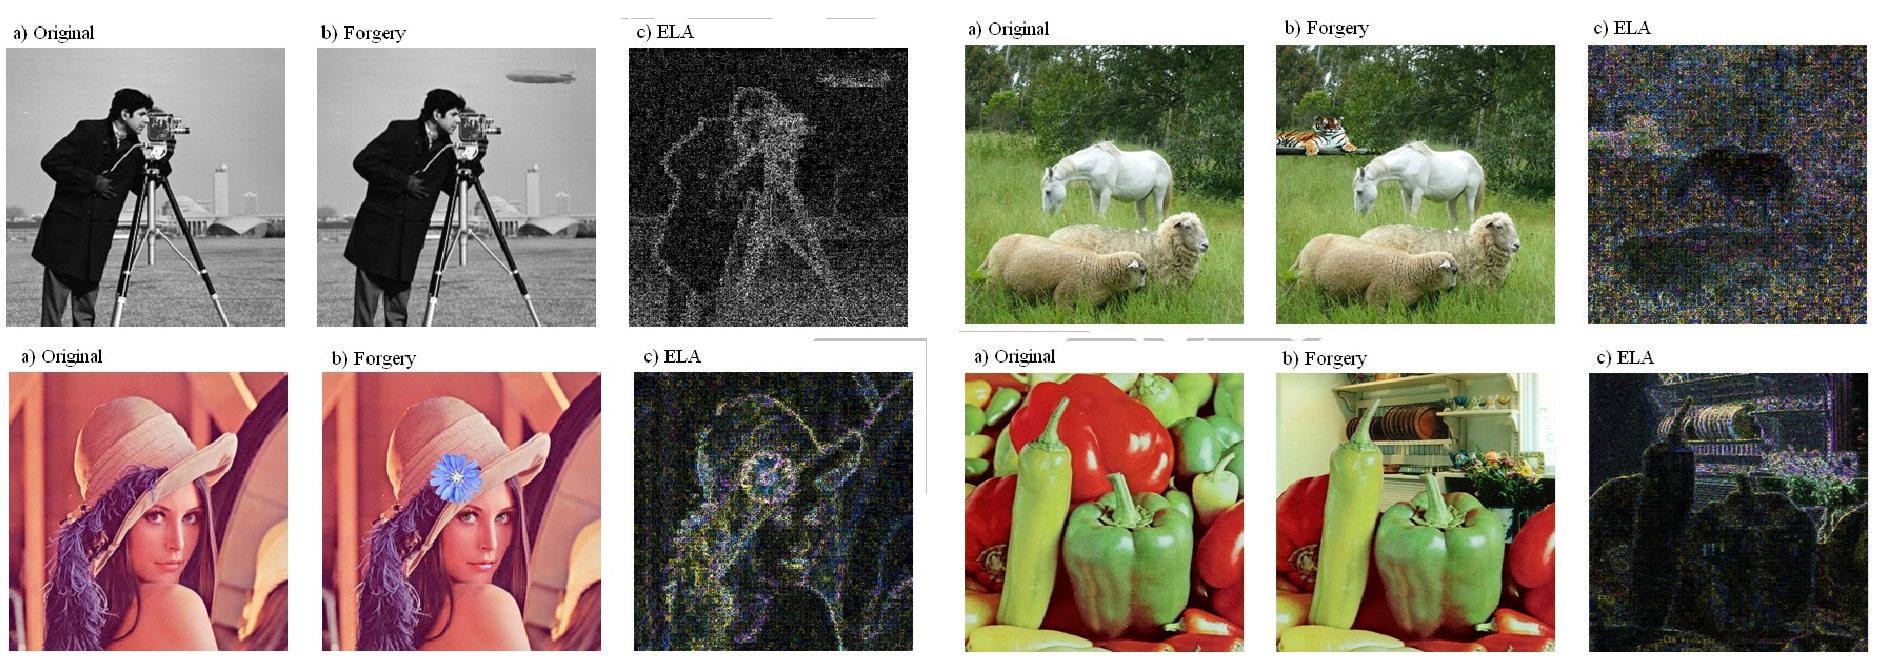
\includegraphics[width=0.8\textwidth]{Pic/ELA_FULL.png}
\end{center}
\end{frame}

\begin{frame}{Error level analysis + Deep Learning \cite{rafique2023deep}}
\begin{center}
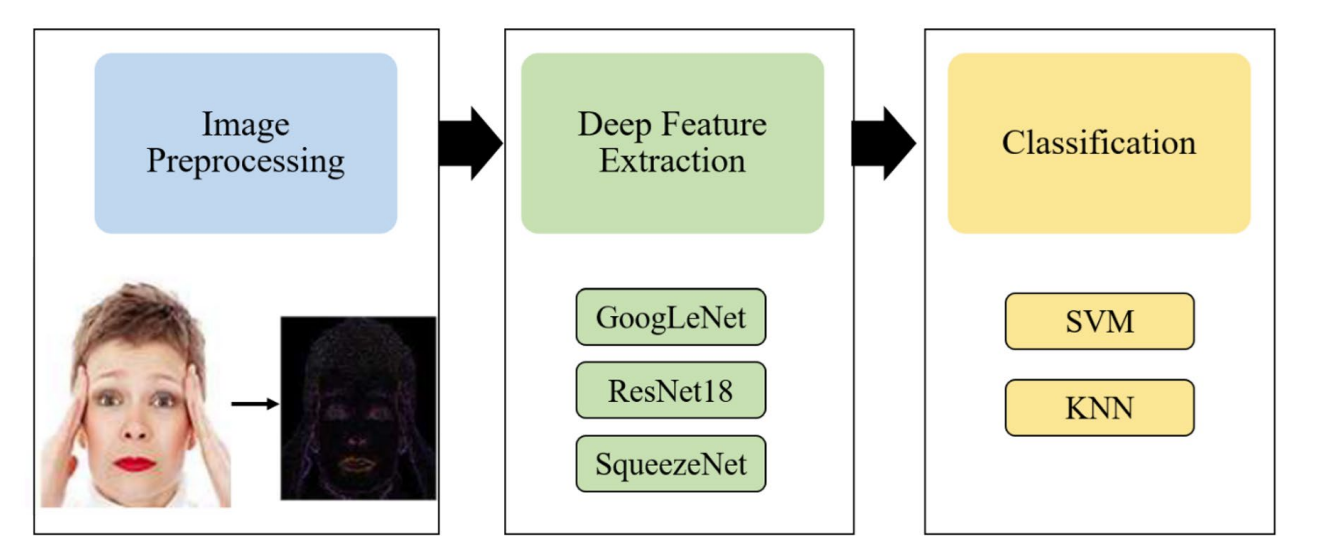
\includegraphics[width=0.8\textwidth]{Pic/ELA+DEEP.png}
\end{center}
\end{frame}

\begin{frame}{Forensically \cite{fr}}
\begin{center}
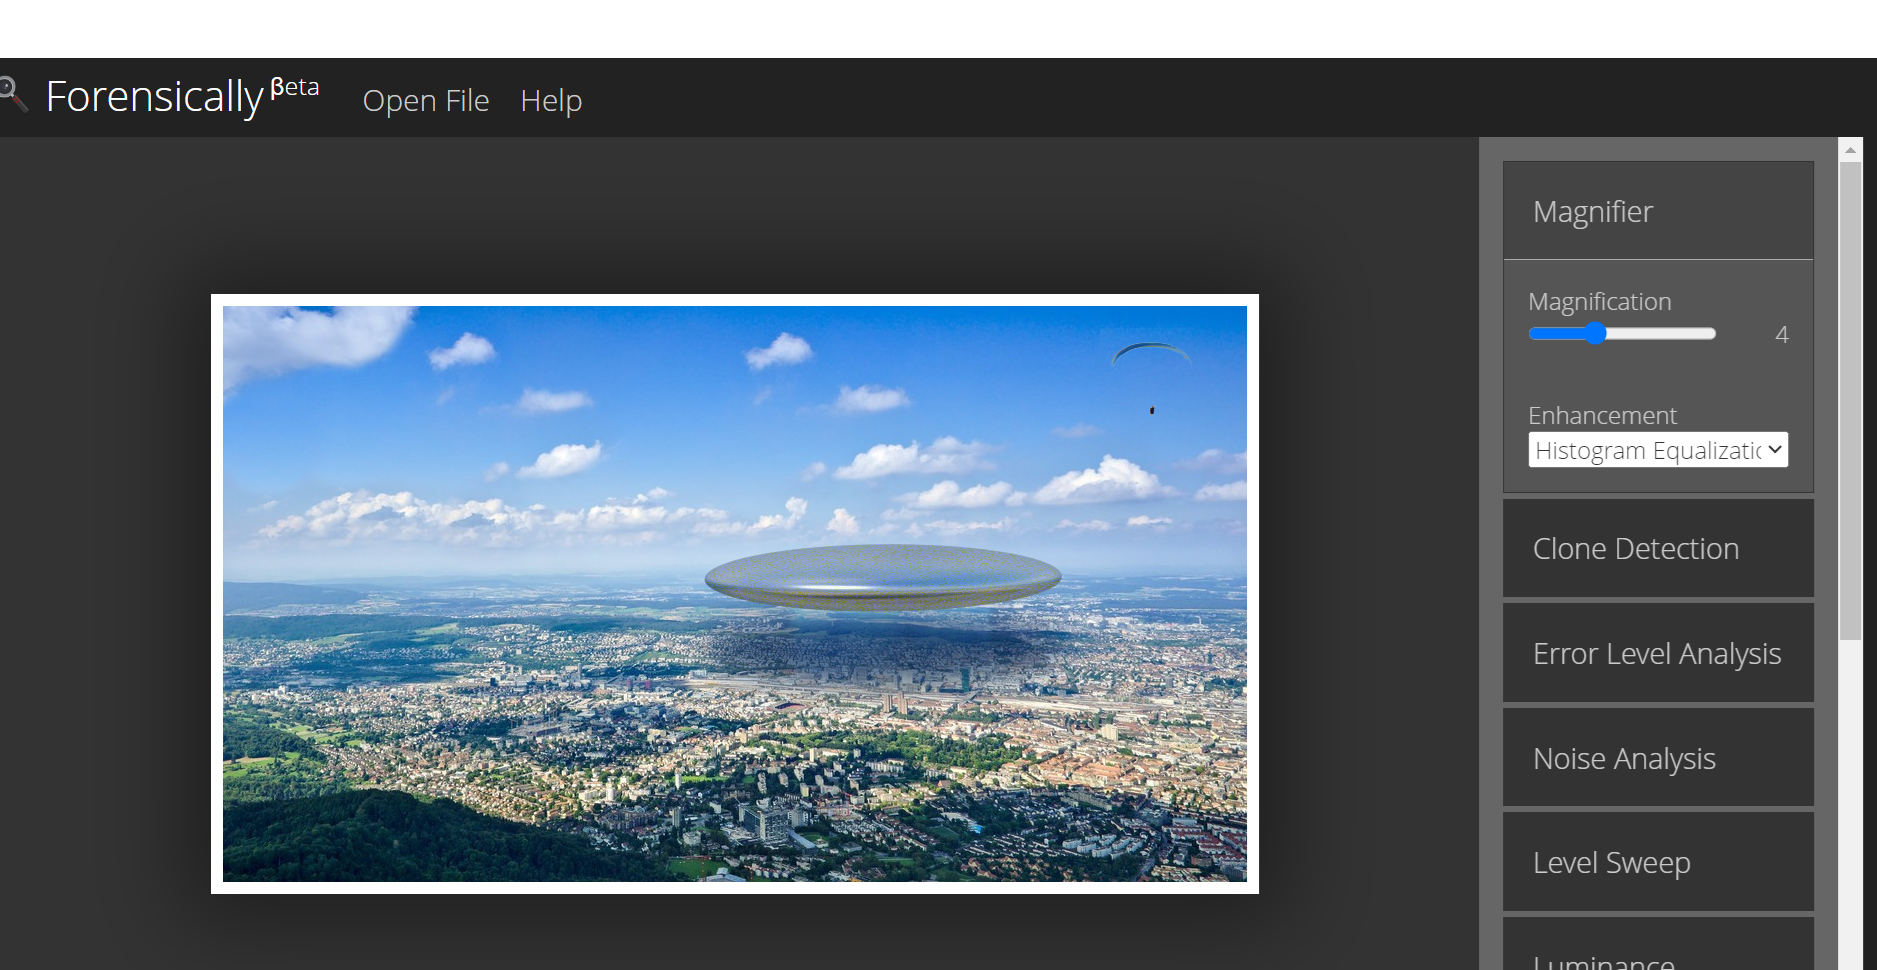
\includegraphics[width=0.8\textwidth]{Pic/forensically.png}
\end{center}
\end{frame}



\section{Aspetti legali}

\begin{frame}
\begin{center}
\Huge
Aspetti legali
\end{center}
\end{frame}



\begin{frame}{IA act, 2024}
\begin{center}
\small
70a) "it is appropriate to require providers of those systems to embed technical solutions that enable \textbf{marking in a machine readable format and detection }that the \textbf{output} has been \textbf{generated or manipulated by an AI} system and not a human"
\end{center}
\end{frame}

\begin{frame}{Conseguenze di un uso improprio dei deepfake \cite{deepfake_jus}}
\begin{alertblock}{Uso improprio dei deepfake}
\begin{itemize}
\item Diffamazione, attraverso la creazione di contenuti che denigrano o danneggiano la reputazione di un individuo
\item Furto di identità, che rileva nel caso della creazione di video o audio in cui un soggetto viene rappresentato come un’altra persona
\item Violazione della privacy, attraverso la condivisione non consensuale di informazioni relative a una persona
\end{itemize}
\end{alertblock}
\end{frame}


\begin{frame}{Tutorial Pratico \cite{foster2022generative}}
\begin{center}
\qrcode[hyperlink,height=.52\textwidth]{https://github.com/marzione00/Lecture_Deepfake/tree/main}
\end{center}
\begin{center}
\url{https://github.com/marzione00/Lecture_Deepfake/tree/main}
\end{center}
\end{frame}








\begin{frame}[t,allowframebreaks]
\frametitle{Bibliography}
\printbibliography
\end{frame}





\end{document}
